% Document releated
% \documentclass[12pt]{report}
%\RequirePackage[T1]{fontenc}
%\RequirePackage[utf8]{inputenc}
%\RequirePackage{environ}

\documentclass[12pt, numbers=noenddot, bibliography=totoc, headings=openright, twoside=semi]{scrbook}
\usepackage[utf8]{inputenc}
\usepackage[T1]{fontenc}
\usepackage{lmodern}
\usepackage[catalan]{babel}
\usepackage{afterpage}

% Configuration of KOMA-script
\setkomafont{dictumtext}{\itshape\small}
\setkomafont{dictumauthor}{\normalfont}
\renewcommand*\dictumwidth{0.75\linewidth}
\renewcommand*\dictumauthorformat[1]{\vspace{0.5cm}--- #1\vspace{0.25cm}}
\renewcommand*\dictumrule{}

% Table of contents depth
\setcounter{tocdepth}{2}

% Cover configuration commands
\def\title#1{\gdef\@title{#1}\gdef\thetitle{#1}}
\def\subtitle#1{\gdef\@subtitle{#1}\gdef\thesubtitle{#1}}
\def\author#1{\gdef\@author{#1}\gdef\theauthor{#1}}
\def\advisor#1{\gdef\@advisor{#1}\gdef\theadvisor{#1}}

% Graphics
\usepackage[labelsep=endash]{caption}
\usepackage{graphicx}
\usepackage{tikz}
\usepackage{newfloat}
\usepackage{subcaption}
\setlength{\abovecaptionskip}{10pt}
\setlength{\belowcaptionskip}{10pt}
\renewcommand{\thesubtable}{\roman{subtable}}
\renewcommand{\thesubfigure}{\roman{subfigure}}
\newenvironment{code}{\captionsetup{type=listing}}{}

% Symbols and Math
\usepackage{amssymb}
\usepackage{amsmath}

% Horizontal lists
\usepackage{tasks}

% Code listings
\usepackage{listings}
\lstset{
  breaklines=true,
  basicstyle=\ttfamily
}
\lstset{columns=fullflexible,basicstyle=\ttfamily}
\usepackage{minted}
%\usemintedstyle{colorful}
\setminted{breaklines=true, baselinestretch=1}
%\DeclareBoolOption{newfloat}

% References and links
\PassOptionsToPackage{hyphens}{url}\usepackage{hyperref}
\addto\extrasenglish{\renewcommand{\chapterautorefname}{Chapter}}
\providecommand*{\listingautorefname}{Listing}
\renewcommand{\lstlistingname}{Listing}
\hypersetup{hidelinks=true}
\usepackage[usestackEOL]{stackengine}

% Custom tab command
\newcommand\tab[1][10mm]{\hspace*{#1}}

% Tables configuration
\setlength{\tabcolsep}{0.6em}
{\renewcommand{\arraystretch}{1.35}

% Footnotes
\renewcommand{\thefootnote}{\textbf{\arabic{footnote}}}
\addtolength{\footnotesep}{1.5mm}
\setlength{\skip\footins}{1cm}

% Bibliography
\usepackage[
    backend=bibtex,
    style=alphabetic,
    citestyle=alphabetic
]{biblatex}
\addbibresource{references}
\nocite{*}

% Headers and footers
\usepackage{fancyhdr,lastpage}
\pagestyle{fancy}
\fancyhf{}
% \renewcommand{\chaptermark}[1]{\markboth{\MakeUppercase{\thechapter.\ #1}}{}}
\renewcommand{\headrulewidth}{0pt}
\renewcommand{\footrulewidth}{0pt}
\fancypagestyle{plain}{
\fancyhf{}
\fancyfoot[RO,LE]{\textit{\thepage}}}
% Identations and newlines
\usepackage[parfill]{parskip}
\usetikzlibrary{
    automata,calc,trees,positioning,arrows,chains,shapes.geometric,
    decorations.pathreplacing,decorations.pathmorphing,shapes,
    matrix,shapes.symbols
}
\tikzset{
    block/.style={rectangle, rounded corners, minimum height=3em, draw=black, very thick,, text centered ,text width=7.5em},
    square/.style={rectangle, draw=black, thick,, text centered},
    big_block/.style={rectangle, rounded corners, minimum height=3em, draw=black, very thick,, text centered ,text width=10em},
    bigger_block/.style={rectangle, rounded corners, minimum height=3em, draw=black, very thick,, text centered ,text width=15em},
    line/.style={->, thick,shorten >=1.5pt},
    dot_arrow/.style={*->, thick, shorten >=1.5pt},
    decoration={brace},
    tuborg/.style={decorate},
    tubnode/.style={midway, right=2pt},
}
%\DeclareQuoteAlias{spanish/spanish}{catalan}
\DeclareFixedFont{\helvbupc}{T1}{phv}{bx}{u}{2cm}
\DeclareFixedFont{\smallhelvbupc}{T1}{phv}{bx}{u}{1.8cm}
\DeclareFixedFont{\helvupc}{T1}{phv}{m}{u}{2cm}
% El color principal, Pantone 3005
\definecolor{upcblue}{HTML}{007AC9}
% bola upc de 10cm
\def\bola@upc{
    \fill [fill=upcblue]  (0,0) circle (5);
    \foreach \x in {-1.8,0,1.8}
    \foreach \y in {-1.8,0,1.8}
    {
      \fill [fill=white,yshift=1cm] (\x,\y) circle (.7);
    }
    \draw [color=white,text centered,font=\helvbupc,yshift=0.2cm]
      (-1.8,-3  ) node {U}
      (0,-3)      node {P}
      (1.8,-3)    node {C};
}

% bola upc amb les lletres centrades a sota
\def\bola@upc@text{
  \bola@upc
  \draw [color=upcblue,text centered,font=\helvupc]
      (0,-7) node {UNIVERSITAT POLIT\`ECNICA DE CATALUNYA};
}

% comanda
\newcommand{\bolaupctext}[1][1cm]{\resizebox{!}{#1}{\tikz\bola@upc@text;}}

\graphicspath{{images/}}

\title{Gestió automatitzada d'un pàrquing}
\subtitle{AppArkem}
\author{Gemma Rosell Guilella}
\advisor{Aleix Llusà Serra}


\begin{document}
\pagestyle{plain}

% Cover
\begin{titlepage}
    \begin{center}
        \resizebox{!}{1.5cm} {
            \begin{tikzpicture}
                \fill [fill=upcblue]  (0,0) circle (5);
                \foreach \x in {-1.8,0,1.8}
                \foreach \y in {-1.8,0,1.8}
                {
                    \fill [fill=white,yshift=1cm] (\x,\y) circle (.7);
                }
                \draw [color=white,text centered,font=\helvbupc,yshift=0.2cm]
                    (-1.8,-3  ) node {U}
                    (0,-3)      node {P}
                    (1.8,-3)    node {C};
                \draw [color=upcblue,text centered,font=\helvupc]
                    (0,-7) node {UNIVERSITAT POLIT\`ECNICA DE CATALUNYA};
            \end{tikzpicture}
        }
        \par
        \textsf{\color{upcblue}\Large Escola Superior d'Enginyeria de Manresa}
        \end{center}
        \vfill
        \begin{center}
        \rule{0.9\textwidth}{1pt}\par
        \noindent\Huge\textbf{\thetitle}\par
        \bigskip\noindent\LARGE\thesubtitle\par
        \bigskip\bigskip
        \large\today\par
        \rule{0.9\textwidth}{1pt}\par

        \vfill
        \Large
        {\scriptsize
            Treball de fi de grau que presenta
        }\\
        \textsc{\theauthor}\\
        {\scriptsize
            en compliment dels requisits per assolir el
        }\\
        \textsc{Grau d'ENGINYERIA EN SISTEMES TIC}
        \par
        \bigskip\large
        {
            Direcció: \theadvisor
        }\\
    \end{center}
\end{titlepage}
\clearpage
% License
\thispagestyle{empty}
\begin{center}

\includegraphics{license}\\
This work is licensed under the Creative Commons Attribution-NonCommercial-ShareAlike 4.0 International License.
To view a copy of this license, visit \url{https://creativecommons.org/licenses/by-nc-sa/4.0/}.
\end{center}



\frontmatter

% Dedication
% \newpage
% \hspace{0pt}
% \vfill
% \thispagestyle{empty}
% \dictum[William Gibson, \textit{Zero History}]{
%     ``When you want to know how things really work, study them when they’re coming apart.''}
% \vfill
% A la meva família i molts amics que em van animar i em van donar suport durant tots aquells anys de carrera.

% \hspace{0pt}
% \afterpage{\null\thispagestyle{empty}\newpage}

% Acknowledgements
\newpage
\hspace{0pt}
\vfill
\thispagestyle{empty}
\centerline{\textbf{Agraïments}}
Vull agrair al director del projecte Aleix Llusà Serra, que m'ha ajudat en el seu desenvolupament
donant-me pautes per l'assoliment de l'objectiu i en la realització de la memòria.
També vull reconèixer l'ajut dels membres del departament de DIPSE, en especial a l'Arnau Arumí per la seva
ajuda, paciència en l'elaboració del projecte i les connexions de la Raspberry Pi amb l'ordinador.

Finalment, donar gràcies a la meva família i els amics que m'han animat i ajudat al llarg
d'aquest projecte, com també durant els anys cursant la carrera.
\vfill
\hspace{0pt}
\afterpage{\null\thispagestyle{empty}\newpage}

% Abstract
\newpage
\hspace{0pt}
\vfill
\setcounter{page}{1}
\phantomsection
\addcontentsline{toc}{chapter}{Resum}
\centerline{\textbf{Resum}}
Aquest projecte consisteix en el disseny i el desenvolupament d'\emph{Apparkem},
una aplicació per a la gestió automatitzada d'un pàrquing inte\l.ligent.
S'introdueix la creació d'un servidor back-end, el front-end de l'aplicació
i una Raspberry Pi que actua com a barrera. Finalment, s'observen els resultats
obtinguts com també possibles propostes de millora per l'aplicació.
\vfill
\phantomsection
\addcontentsline{toc}{chapter}{Abstract}
\centerline{\textbf{Abstract}}
This project consists of the design and development of \emph{Apparkem}, an application
for the automated smart parking management. It introduces the creation
of a back-end server, the front-end of the application and a Raspberry Pi that
acts as a barrier. Finally, the results obtained are observed as well as possible
improvement proposals for the application.




\vfill
\hspace{0pt}
\afterpage{\null\thispagestyle{empty}\newpage}

\tableofcontents
\listoffigures
\listoftables
% \listoflistings

\mainmatter

\clearpage
% \renewcommand{\chaptermark}[1]{\markboth{\MakeUppercase{\thechapter.\ #1}}{}}
% \renewcommand{\sectionmark}[1]{\markright{\ #1}{}}
\fancyhead[L]{\scriptsize{\textsl{\leftmark}}}
\fancyhead[R]{\scriptsize{\textsl{\rightmark}}}

\part{Memòria}

% Capitols memòria
\chapter{Introducció}

Aquest projecte consisteix en dissenyar una aplicació per a la gestió automatitzada d'un pàrquing inte\l.ligent.
Aquest control es basa en l'entrada i sortida de vehicles d'aquest pàrquing fent servir altres alternatives
al lector de matrícules convencional. A més a més, l'aplicació tindrà un registre de l'estança de cada usuari,
com també la part de configuració pels treballadors.

Algunes d'aquestes alternatives són la comunicació Bluetooth i els codis QR.
En aquest projecte se centra a crear una aplicació on s'utilitza els codis QR.

També, aquesta aplicació dóna l'eina perquè l'usuari faci els pagaments a través d'ella d'una manera segura.

\section{Objectius}

L'objectiu es pot dividir en els punts següents:

\begin{itemize}
    \item Buscar informació sobre els generadors i lectors dels codis QR, com també dels lectors de matrícules i la comunicació Bluetooth.
    \item Aprendre a dissenyar un \emph{backend} i un \emph{frontend}.
    \item Aprendre tots els passos que comporta la creació d'una aplicació i fer-los segons les necessitats del projecte.
    \item Dissenyar un sistema on emmagatzemar les dades, una base de dades. Aprendre MySQL.
    \item Dissenyar l'aplicació perquè l'usuari tingui un bon aprenentatge quan entri per a primer cop, aquesta tingui una eficiència excepcional i sobretot hi hagi seguretat.
    \item Triar dues framework per al desenvolupament de l'aplicació, una per el \emph{backend} i l'altre per el \emph{frontend}.
    \item Aprendre els passos de la framework de React, com també la del Laravel.
\end{itemize}

\section{Conceptes previs}

\begin{itemize}
    \item El \emph{back-end} és la capa d'accés a les dades, és la lògica que fa que una pàgina web funcioni,
    cosa que queda amagada als ulls de l'usuari. Determina que tan bé s'executarà l'aplicació i quina
    experiència obtindrà l'usuari del seu ús, positiva o negativa.
    Es fan servir habitualment llenguatges com PHP, Javascript, Python i Ruby, entre d'altres.
    \item El \emph{front-end} és la part del desenvolupament que es dedica el disseny,
    des de l'estructura del lloc fins als estils com colors, fons, mides fins a arribar a les animacions i efectes.
    És aquesta part de la pàgina amb què interaccionen els usuaris, és tot el que el visitant veu i experimenta
    de manera directa.
    \item \emph{MySQL} és un sistema de gestió de bases de dades relacional que usa el llenguatge SQL per comunicar-s'hi. Algunes
    d'aquestes comunicacions poden ser consultar les dades, manipular-les, etc.
    \item Una \emph{framework} és una eina de desenvolupament web que ens permet desenvolupar aplicacions d'una
    manera més àgil utilitzant les seves llibreries i funcionalitats. Ajuda als programadors a seguir una estructura,
    estalviar temps i esforços, ja que d'aquesta manera es centrin a buscar solucions a nous problemes i a <<No reinventar la roda>>.
    \item \emph{React} \autocite{react} és una llibreria de JavaScript per desenvolupar interfícies d'usuari.
    \item \emph{Laravel} \autocite{laravel} és una framework del llenguatge de programació PHP.
    S'utilitza per al desenvolupament d'aplicacions web.
\end{itemize}

\newpage
\section{Alternatives per l'accés al pàrquing}
\label{sec:alternatives}

En aquest apartat s'avaluen tres metodologies
diferents per a poder control l'accés al pàrquing que són el lector de
matrícules, la connexió Bluetooth i els codis QR.

\subsection{Lectors de matrícules}
Els sistemes de lectors de matrícula són
especialment utilitats gràcies a la seva fàcil insta\l.lació i la fiabilitat de
la lectura. Alguns exemples on es poden trobar és en el control de pàrquings i
els controls de trànsit.

\subsubsection{Funcionament}

\begin{itemize}
    \item Captar en una imatge la matrícula a través d'una càmera.
    \item El software fa una interpretació d'aquesta imatge.
    \item S'inclouen les dades interpretades en una base de dades.
\end{itemize}

Els lectors de matrícules permeten transformar una imatge presa
des d'una càmera i, mitjançant un procés de visió artificial, a un
paràmetre digital. El sistema és capaç de discriminar l'entorn i
fixar-se només a la placa d'una matrícula, creant un codi únic
per a ella.

\subsubsection{Conclusió}

La seva fiabilitat en la lectura i facilitat de la insta\l.lació
converteix en una eina útil, segura i necessària. Tanmateix, s'ha de tenir present
la resposta ràpida en un possible fet que provoqui un incident i ens desenvolupi un
problema en el nostre pàrquing.

En aquesta projecte, s'estan buscant diferents solucions per poder resoldre aquestes
dificultats.


\newpage
\subsection{Comunicació amb Bluetooth}
Els dispositius Bluetooth es co\l.loquen a les barreres dels pàrquings i
permeten controlar l'entrada i sortida. Es fan ús sobretot en pàrquings
privats o pàrquings d'institucions.

\subsubsection{Funcionament}
\label{sssec:alternatives}

\begin{itemize}
    \item Obtenir el dispositiu i co\l.locar-lo en la barrera del pàrquing.
    \item Una aplicació que serà el comandament del garatge o el tiquet per entrar al pàrquing.
    \item Donar accés a altres persones.
    \item Tenir un registre d'entrades i sortides.
    \item Comunicació amb Bluetooth encriptat.
\end{itemize}


El Bluetooth és un protocol de comunicació que ens permet la transmissió
de dades entre diferents dispositius que es troben a poca distància. La seva transmissió
sense fils es fa través d'ones de ràdio. Per aquesta raó els dispositius han d'estar
lleugerament a prop. Aquests dispositius es poden classificar segons la seva potència i
distància de detecció.

\subsubsection{Conclusió}

Per acabar, els dispositius Bluetooth tenen un paper important en garatges privats o en els pàrquings. Actualment, ja existeixen alguns dispositius
que fan aquest servei, ja que s'insta\l.la un dispositiu junt amb la barrera d'accés i a través aquesta
tecnologia es connecta amb el dispositiu mòbil, que aquest actua com a comandament per poder entrar o sortir
d'aquest. És bastant utilitzat en garatges privats o pàrquings d'institucions privades on el personal és conegut.

\newpage
\subsection{Introducció codi QR}
Els codis QR (Quick Response code) són un tipus de
codis de barres de dues dimensions en forma de matriu que permeten emmagatzemar informació.
La seva forma quadrada és caracteritzada per tres quadres situats a les cantonades superiors
i inferiors. La mida de la imatge depèn de la quantitat d'informació que aquest emmagatzema.

\begin{figure}[H]
    \begin{center}
      
\includegraphics[scale=0.50]{Fotos/BenvingutsCodiQR.png}
    \end{center}
    \caption{Exemple d'un Codi QR}
    \label{fig:compiler_phases}
  \end{figure}

La utilització inicial dels codis QR tenia com a objectiu principal en la indústria de l'automoció.
Actualment, la possibilitat de llegir els codis QR és existent. Per exemple els telèfons mòbil permeten l'ús d'aquests
codis en una infinitat d'aplicacions. Una de les raons principals són perquè aquests codis poden interactuar fàcilment amb
un dispositiu mòbil i realitzar accions. En l'actualitat, a causa de la Covid-19, s'ha fet un gran ús d'aquesta eina.
Per exemple llegir un URL d'una pàgina web per descarregar-nos la carta o el menú d'un restaurant.

\subsubsection{Estructura Codi QR}

En aquest subapartat es fa referència a l'estructura i les especificacions del codi QR.

\begin{itemize}
  \item \emph{Marques d'orientació}: són els patrons de posició i els d'alineació.
  Estan situades als extrems del codi QR. S'utilitzen per saber l'orientació del codi.
  Poden variar depenent de la dimensió del codi QR.
  \begin{itemize}
    \item \emph{Patrons de posició}: Són tres quadrats que estan als extrems del codi QR.
    \item \emph{patrons d'alineació}: S'usen per a la detecció de la posició.
  \end{itemize}
  \item \emph{Informació del format}: S'empra per saber quin nivell d'error i quina màscara s'ha aplicat en el codi.
  \item \emph{Mètrica}: Igual a tots els codis QR i és feta servir per identificar els punts blancs i negres de la matriu.
  \item \emph{Dades}: Les dades s'emmagatzemen en \emph{codewords} de mòduls. Els \emph{codewords} són conjunts de 8 bits que varien la seva forma.
  N'hi ha de dos tipus, el d'informació i el de correcció d'errors. Les dades que hi ha tenen uns bits dedicats a especificar
  el format de les dades, i la quantitat de caràcters que hi ha en el QR. Actualment, els QR accepten diferents formats per a les dades.
  \item \emph{Codis correcció d'errors}: Proporcionen la capacitat de correcció dels codis QR, que s'expressa en un percentatge i correspon
  al tant per cent de dades que es podrà recuperar en cas d'error. Actualment, hi ha 4 nivells de correcció pels codis QR:
  \begin{itemize}
  \item L 7\%
  \item M 15\%
  \item Q 25\%
  \item H 30\%
  \end{itemize}
  \item \emph{Informació de la versió}: Conté la informació de la versió que s'està fent servir. Situada en els laterals
  de dins de les marques d'orientació.
  \item \emph{Sense ús}: Es troben en algunes versions dels codis QR, l'últim \emph{codeword} dels codis d'error no es fa servir.
\end{itemize}

\begin{figure}[H]
    \begin{center}
      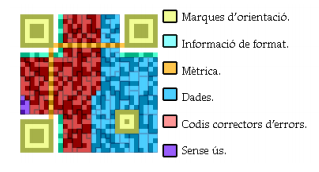
\includegraphics[scale=1]{Fotos/EstructuraCodiQR.png}
    \end{center}
    \caption{Estructura dels Codis QR}
    \label{fig:compiler_phases}
  \end{figure}

\subsubsection{Generar Codi QR}

En aquest projecte l'encarregat de fer el codi QR i mostrar-lo als usuaris és el \emph{front-end} de l'aplicació. Encara que
l'encarregat de generar el text és el servidor. \autoref{chap:back-end}

\subsubsection{Lectura Codi QR}


En aquest projecte l'encarregat de fer la lectura del QR és la Raspberry Pi actuant com a barrera fent servir una càmera.
\autoref{chap:raspberryPi}

\section{Altres aplicacions}
De les diferents alternatives que s'ha explicat en el capítol anterior \autoref{sec:alternatives}
existeixen diferents aplicacions que hi ha al mercat que solucionen el problema real
són les següents:

\begin{enumerate}
    \item \texttt{telpark}: Una aplicació amb la possibilitat de reservar una plaça de pàrquing posar el pàrquing on es vol
    aparcar, posar la durada amb possibilitat d'augmentar el temps, el vehicle i la forma de pagament.
    Possibilitat de pagar el parquímetre \autocite{telpark}.
    \item \texttt{Parkingdoor}: Aquesta aplicació és útil en garatges privats, quan es vol estalviar el comandament
    per pujar la porta del garatge. S'ha d'insta\l.lar un dispositiu junt la porta i el dispositiu mòbil que actua
    com a comandament. Com s'ha explicat en l'apartat de \autoref{sssec:alternatives}.
    Més informació a \autocite{parkingdoor}.
    \item \texttt{El Parking}: Aquesta aplicació dóna la possibilitat de fer pagaments a través de l'aplicació.
    Fer reserves amb la possibilitat de cance\l.lació. Més informació a \autocite{el_parking}.
\end{enumerate}

Totes aquestes aplicacions tenen la característica de funcionar amb diferents pàrquings a la vegada.
L'aplicació d'aquest projecte es basa en la creació de la gestió d'un pàrquing privat, d'una institució o la
possibilitat de ser un pàrquing públic. On la configuració d'aquests és única i personal, és a dir, l'aplicació és feta a mida per
a cada un dels pàrquings. A més a més, amb la funcionalitat d'usar els codis QR per les entrades i sortides del pàrquing.

\chapter{Arquitectura del sistema}
L'arquitectura del projecte consta en tres parts:
\begin{itemize}
    \item Un ordinador amb un servidor de Laravel, que és el \emph{back-end}.
    \item El \emph{front-end} de l'aplicació utilitzant la llibreria de React.
    \item Una Raspberry Pi que actua com a barrera del pàrquing.
\end{itemize}

\begin{figure}[H]
    \begin{center}
        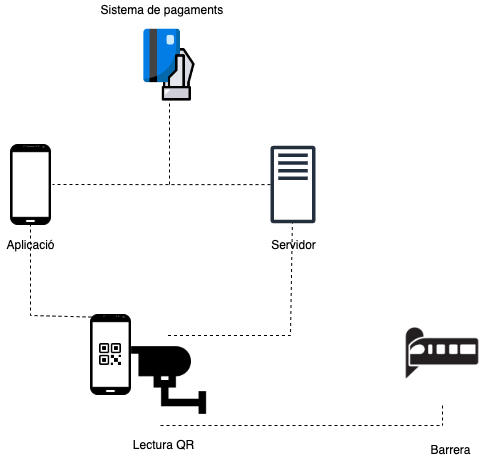
\includegraphics[scale=0.60]{Fotos/arquitectura_sistema.png}
    \end{center}
    \caption{Arquitectura del sistema}
    \label{fig:compiler_phases}
\end{figure}

\newpage
\section{Back-end}

L'arquitectura que utilitza la \emph{framework} de Laravel es basa en el MVC (Model-Vista-Controlador),
feta servir per la implementació d'interfícies d'usuari, dades i la lògica.
Aquesta separació ens dóna una millor divisió de treball i millora el manteniment.
\begin{itemize}
    \item Model: és qui defineix quines dades ha de tenir l'aplicació i les modifica. Si aquestes canvien, notifiquen a la vista.
    \item Vista: com s'han de mostrar les dades a l'aplicació per a l'usuari, és el disseny i la presentació.
    \item Controlador: on conté la lògica que actualitza el model. És la resposta a la so\l.licitud que fa l'usuari.
    Es comunica amb el model.
\end{itemize}

\begin{figure}[H]
    \begin{center}
        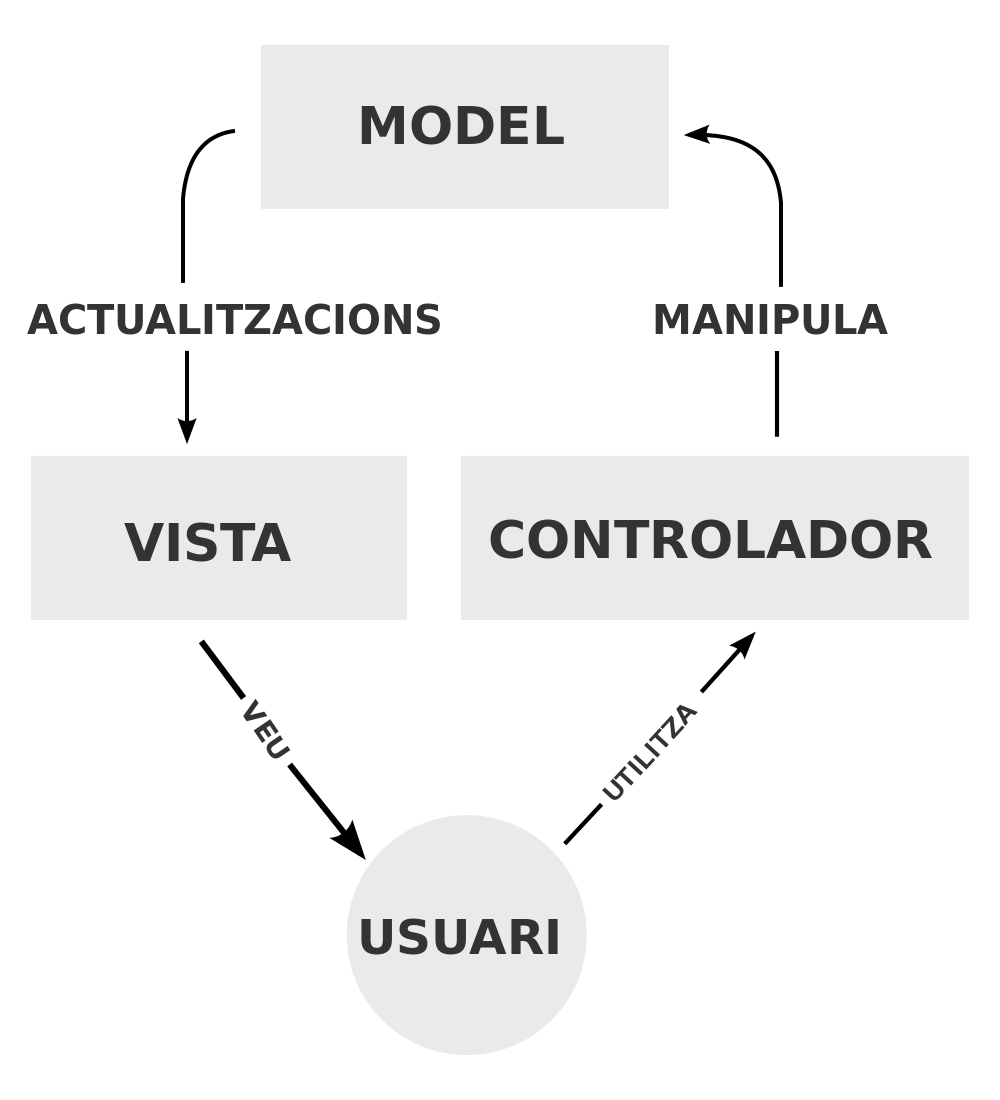
\includegraphics[scale=0.20]{Fotos/arquitectura_mvc.png}
    \end{center}
    \caption{Relació entre els elements del model MVC \autocite{mvc}}
    \label{fig:compiler_phases}
\end{figure}

\section{Front-end}

El \emph{front-end} conjuntament amb la llibreria de React la qual crea components independents
que cada un d'ells és una peça on l'usuari pot interactuar. S'encarrega de crear un espai personal
per l'usuari. Generar els diferents codis QR per l'accés o la sortida del pàrquing.
Mostrar la informació sobre l'aparcament. Fer pagaments d'una forma senzilla i amb seguretat.
A més a més disposa d'un apartat per l'administració on hi ha una part de configuració i un recull de dades.

\section{Barrera}

La Raspberry Pi a través de la càmera s'encarrega de detectar diferents codis QR. Aquests, són els
que s'han generat amb l'aplicació del \emph{front-end}. Aquesta detecció implica que la barrera
actuï de diferent manera, pujant-la o baixant-la en funció del tipus del codi QR generat.
Per aconseguir aquest efecte s'ha emprat una màquina d'estats \autocite{maq_estats}.

\chapter{Back-end}
\label{chap:back-end}

En aquest capítol es fa referència a la implementació del \emph{back-end} de la aplicació.
Està implementat amb la framework de \texttt{Laravel} \autocite{laravel}
és una framework del llenguatge de programació PHP. S'utilitza per al desenvolupament d'aplicacions web.

\section{Elecció de l'entorn}

En aquesta secció s'explica els punts forts de la eina triada per realitzar el \emph{back-end} de l'aplicació.

\begin{itemize}
    \item És una de les frameworks més utilitzades \autocite{estadistiques_backend}.
    \item L' \texttt{ecosistema}, és a dir la comunitat que hi ha fent-ne ús cada dia.
    Facilita a l'hora de trobar solucions a problemes que es poden trobar al llarg del
    desenvolupament d'una aplicació. També ajuda al fet que sigui una eina on sempre hi
    hagi un manteniment i estigui actualitzada a noves eines per facilitar la feina o fins
    i tot a estalviar-ne.
    \item Laravel inclou \texttt{Eloquent}, mapatge d'objectes relacional (ORM) que fa que sigui
    agradable interactuar amb la base de dades. Cada taula de base de dades té un "Model"
    corresponent que s'utilitza per interactuar amb aquesta taula. A més de recuperar registres
    de la taula de la base de dades, també permeten inserir, actualitzar i eliminar registres
    de la taula \autocite{eloquent_laravel}.
    \item \texttt{Recursos API}, Quan l'aplicació crea una API, és possible que necessiti una capa
    de transformació que es trobi entre els models Eloquent i les respostes JSON que realment
    es retornen als usuaris de l'aplicació. Permet transformar de manera expressiva i senzilla
    els models i co\l.leccions de models en JSON.
    Ofereixen un control més sòlid sobre la serialització JSON dels models i les seves relacions
    \autocite{resources_laravel}.
    \item Una altra eina són les \texttt{migracions}, permet definir i compartir l'esquema de la
    base de dades de l'aplicació \autocite{migrations_laravel}.
    \item L'\texttt{Autenticació}, Laravel s'esforça per oferir les eines necessàries per implementar
    l'autenticació de manera ràpida, segura i senzilla \autocite{auth_laravel}.
    \item Sistema de \texttt{caché} fa que l'aplicació vagi igual de ràpid en local que en producció.
    \item La \texttt{validació de dades}: Laravel ofereix diversos enfocaments diferents per validar
    les dades entrants de l'aplicació, les so\l.licituds HTTP entrants. Inclou una gran varietat de
    regles de validació \autocite{validacio_dades_laravel}.
    \item \texttt{Laravel cashier Stripe} ofereix una interfície expressiva i fluida als serveis de
    facturació de subscripcions de Stripe. Gestiona gairebé tot el codi de facturació de subscripció general i
    d'altres \autocite{cashier_laravel}.
    \item \texttt{Laravel Sanctum} ofereix un sistema d'autenticació lleuger per a SPA
    (aplicacions d'una sola pàgina), aplicacions mòbils i API simples basades en tokens \autocite{sanctum_laravel}.
\end{itemize}

\section{Base de dades}
\label{chap:base_dades}

Qualsevol aplicació interactua amb una base de dades per tal de recopilar i emmagatzemar dades
amb una tècnica ordenada i seguint una estructura coherent i accessible.
Com s'ha esmentat en la secció anterior, Laravel utilitza l'ORM Eloquent.

L'estructura de la base de dades és de la següent manera:

\begin{figure}[H]
\begin{center}
    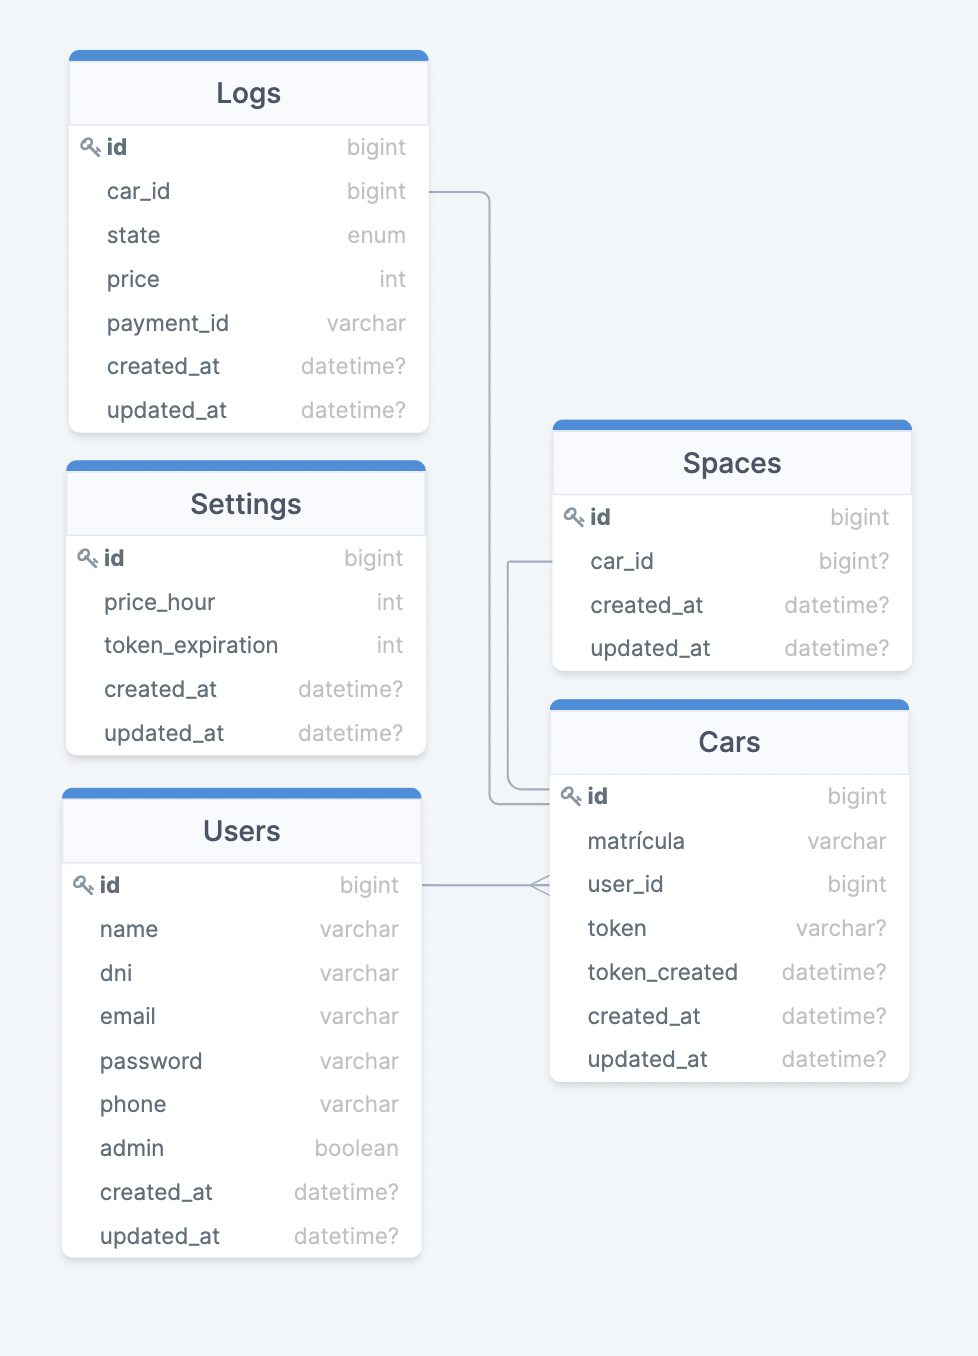
\includegraphics[scale=0.45]{Fotos/BD.png}
\end{center}
\caption{Estructura base de dades}
% \label{fig:BD}
\end{figure}

\begin{table}[H]
\centering
\begin{tabular}{lll}
\hline
\textbf{Columna} & \textbf{Tipus} & \textbf{Descripció}                                                                                             \\ \hline
id               & integer        & \begin{tabular}[c]{@{}l@{}}Clau primària, única per a cada usuari. \\ Autoincrementa el seu valor\end{tabular} \\ \hline
name              & varchar(255)   & Nom i cognom de l'usuari.                                                                                       \\ \hline
dni              & varchar(9)     & \begin{tabular}[c]{@{}l@{}}Número del DNI de cada usuari. \\ Únic per a cada usuari.\end{tabular}               \\ \hline
email            & varchar(255)   & \begin{tabular}[c]{@{}l@{}}Correu electrònic de l'usuari. \\ Únic per a cada usuari.\end{tabular}               \\ \hline
password      & varchar(255)   & \begin{tabular}[c]{@{}l@{}}Contrasenya de l'usuari per poder \\ entrar a l'aplicació.\end{tabular}              \\ \hline
phone & varchar(12) & \begin{tabular}[c]{@{}l@{}}Número de telèfon de l'usuari amb \\ un màxim de 12 caràcters. \\ Únic per a cada usuari.\end{tabular} \\ \hline
admin            & boolean           & \begin{tabular}[c]{@{}l@{}}Indica si la persona és adminstrador. \\ Per defecte sempre serà fals.\end{tabular}  \\ \hline
\end{tabular}
\caption{Taula \emph{Users} de la base de dades}
% \label{tab:my-user-table}
\end{table}

\begin{table}[H]
\centering
\begin{tabular}{lll}
\hline
\textbf{Columna}   & \textbf{Tipus} & \textbf{Descripció}                                                                                                                              \\ \hline
id                 & integer        & \begin{tabular}[c]{@{}l@{}}Clau primària, única per a cada usuari. \\ Autoincrementa el seu valor.\end{tabular}                                  \\ \hline
matrícula          & varchar(7)     & \begin{tabular}[c]{@{}l@{}}Número de matricula del vehicle. \\ Únic per a cada vehicle amb un \\ màxim de 8 caràcters.\end{tabular}              \\ \hline
usuari\char`_id         & bigint         & \begin{tabular}[c]{@{}l@{}}Clau foràna, el seu valor correspon\\ a la ID de la taula d'usuaris.\\ Indica de qui pertany el vehicle.\end{tabular} \\ \hline
token              & varchar(16)    & \begin{tabular}[c]{@{}l@{}}String encriptat de 16 caràcters. Nullable.\\ Serveix per poder construir el codi QR.\end{tabular}                    \\ \hline
token\char`_created\char`_at & datetime       & \begin{tabular}[c]{@{}l@{}}Es guarda en quina data\\ s'ha generat el token anterior.\end{tabular}                                                \\ \hline
\end{tabular}
\caption{Taula \emph{Cars} de la base de dades}
% \label{tab:my-car-table}
\end{table}

\begin{table}[H]
\centering
\begin{tabular}{lll}
\hline
\textbf{Columna} & \textbf{Tipus} & \textbf{Descripció} \\ \hline
id & bigint & \begin{tabular}[c]{@{}l@{}}Clau primària, única per a cada usuari.  \\ Autoincrementa el seu valor\end{tabular} \\ \hline
car\char`_id & bigint & \begin{tabular}[c]{@{}l@{}}Número d'identificador del vehicle\\ que ocupa la plaça. \\ Clau foràna de la taula cotxes. \\ Nullable.\end{tabular} \\ \hline
\end{tabular}
\caption{Taula \emph{Spaces} de la base de dades}
% \label{tab:my-spaces-table}
\end{table}

\begin{table}[H]
\centering
\begin{tabular}{lll}
\hline
\textbf{Columna} & \textbf{Tipus} & \textbf{Descripció} \\ \hline
id & bigint & \begin{tabular}[c]{@{}l@{}}Clau primària, única per a cada usuari. \\ Autoincrementa el seu valor\end{tabular} \\ \hline
price\char`_hour & int & \begin{tabular}[c]{@{}l@{}}Número que indica el preu hora \\ del pàrquing.\end{tabular} \\ \hline
token\char`_expiration & int & \begin{tabular}[c]{@{}l@{}}Número que indica el temps de \\ validesa dels codis QR\end{tabular} \\ \hline
\end{tabular}
\caption{Taula \emph{Settings} de la base de dades}
% \label{tab:my-settings-table}
\end{table}

\begin{table}[H]
\centering
\begin{tabular}{lll}
\hline
    \textbf{Columna} & \textbf{Tipus}          & \textbf{Descripció}                                                                                             \\ \hline
    id               & bigint                  & \begin{tabular}[c]{@{}l@{}}Clau primària, única per a cada usuari.  \\ Autoincrementa el seu valor\end{tabular} \\ \hline
    car\char`_id          & bigint                  & \begin{tabular}[c]{@{}l@{}}Clau foràna de la taula cotxes. \\ Número d'identificador del vehicle.\end{tabular}  \\ \hline
    state            & enum ("enter" o "exit") & \begin{tabular}[c]{@{}l@{}}Indica si el vehicle entra o surt del\\ pàrquing.\end{tabular}                       \\ \hline
    price            & int                     & Preu total que li ha costat al usuari.                                                                          \\ \hline
    payment\char`_id      & varchar(255)            & ID del pagament d'Stripe.                                                                                       \\ \hline
\end{tabular}
\caption{Taula \emph{Logs} de la base de dades}
% \label{tab:my-logs-table}
\end{table}

\newpage
\section{Rest API}

En aquesta secció es fa referència a les REST API que s'han creat a l'aplicació.
La \emph{base endpoint} és \url{https://gemmaguilella.cat/api}.


\subsection{Autentificació}

L'autentificació d'aquest projecte és a través del \emph{Laravel Sanctum} \autocite{sanctum_laravel}.
Aquesta eina ofereix guardar els tokens dels usuaris en una base de dades, aquests han de ser els
mateixos tokens que arriben de l'usuari a les peticions HTTP  en el \emph{Authoritzon header} com a
\emph{Barear Token}.

\begin{table}[H]
\centering
\begin{tabular}{llll}
\hline
\textbf{Mètode} & \textbf{Ruta} & \textbf{Middelware} & \textbf{Descripció} \\ \hline
POST            & /auth/login     & guest &  \autoref{sssec:iniciar_sessio}{ Iniciar sessió}     \\ \hline
POST            & /auth/logout    & guest &  \autoref{sssec:tancar_sessio}{ Tancar sessió}     \\ \hline
POST            & /auth/register  & auth  &  \autoref{sssec:crear_usuari}{ Crear usuari}    \\ \hline
GET             & /auth/user      & auth  &  \autoref{sssec:obtenir_usuari}{ Obtenir usuari}    \\ \hline
PUT             & /auth/user      & auth  &  \autoref{sssec:modificar_usuari}{ Modificar usuari}  \\ \hline
\end{tabular}
\caption{Taula rest API \emph{Auth}}
\label{tab:my-auth-api-table}
\end{table}

El \emph{middelware} auth, vol dir que es passa el \emph{Authorization header} \autocite{middleware_laravel}.

\subsubsection{Iniciar sessió}
\label{sssec:iniciar_sessio}

Un exemple del \emph{body} d'una petició HTTP per realitzar l'inici de sessió és enviar
el següent JSON:

\begin{minted}{json}
{
    "email": "gemma@guilella.cat",
    "password": "Password123!"
    "device_name": "web"
}
\end{minted}

El serviodr pot respondre amb les dades del usuari junt amb un \emph{token} identicatiu que es necessita per
autentificar futures peticions HTTP:
\begin{minted}{json}
{
    "token": "10|6MT6IDkmuMqYGDzCg4SwuVcAczASx2BI5prpZiUe",
    "user": {
        "id": 2,
        "name": "Gemma",
        "email": "gemma@guilella.cat",
        "dni": "39393939B",
        "phone": "34625664404",
        "admin": false
    }
}
\end{minted}


\subsubsection{Tancar sessió}
\label{sssec:tancar_sessio}

Per realitzar la petició de HTTP per tancar la sessió és enviar aquesta informació.
En format JSON és el següent:
\begin{minted}{json}
{
    "device_name": "web"
}
\end{minted}


\subsubsection{Crear usuari}
\label{sssec:crear_usuari}

Un exemple del \emph{body} d'una petició HTTP per realitzar registre d'usuaris és enviar
el següent JSON:
\begin{minted}{json}
{
    "name": "Gemma",
    "email": "gemma@guilella.cat",
    "dni": "39393939B",
    "password": "Password123!"
    "password_confirmation": "Password123!"
    "phone": "34625664404",
    "device_name": "web"
}
\end{minted}

La resposta amb JSON del servidor posterior d'enviar el passat exemple és amb les dades del usuari
junt amb el \emph{token} identicatiu de l'usuari.
\begin{minted}{json}
{
    "token": "10|6MT6IDkmuMqYGDzCg4SwuVcAczASx2BI5prpZiUe",
    "user": {
        "id": 2,
        "name": "Gemma",
        "email": "gemma@guilella.cat",
        "dni": "39393939B",
        "phone": "34625664404",
        "admin": false
    }
}
\end{minted}

\subsubsection{Obtenir usuari}
\label{sssec:obtenir_usuari}

Un exemple de la petició HTTP per obtenir la informació d'un usuari és enviar
en els \emph{headers} el \emph{token} de l'usuari.
\begin{minted}{json}
{
    "Authorization": "Bearer 16|89pozuuct0qgewfAPuZR0Ocu3hMSmkuUU0KzpdDz"
}
\end{minted}

La resposta del servidor a la petició HTTP anterior és donar la informació
de l'usuari.
\begin{minted}{json}
{
    "admin": false
    "dni": "39393939B"
    "email": "gemma@guilella.cat"
    "id": 2
    "name": "Gemma Rosell Guilella"
    "phone": "+34625664404"
}
\end{minted}


\subsubsection{Modificar usuari}
\label{sssec:modificar_usuari}

Un exemple del \emph{body} d'una petició HTTP per modificar la informació d'un usuari és enviar
en el següent JSON:
\begin{minted}{json}
{
    "name": "Gemma Rosell Guilella",
    "dni": "39393939B",
    "password": "Password124!"
    "password_confirmation": "Password124!"
    "phone": "34625664404",
    "device_name": "web"
}
\end{minted}

La resposta del servidor a la petició HTTP anterior és donar la informació del usuari.
Seguint l'exemple anterior, el JSON de la resposta és el següent:
\begin{minted}{json}
{
    "admin": false
    "dni": "39393939B"
    "email": "gemma@guilella.cat"
    "id": 2
    "name": "Gemma Rosell Guilella"
    "phone": "+34625664404"
}
\end{minted}

\subsection{Barreres}

% POST            api/barriers/open ................................ barriers.open › BarrierController@open

\begin{table}[H]
\centering
\begin{tabular}{lll}
\hline
\textbf{Mètode} & \textbf{Ruta} & \textbf{Descripció} \\ \hline
POST            & /barriers/open &  \autoref{sssec:pujar_barrera}{ Pujar barrera}     \\ \hline
\end{tabular}
\caption{Taula rest API \emph{Barriers}}
\label{tab:my-barriers-api-table}
\end{table}

\subsubsection{Pujar barrera}
\label{sssec:pujar_barrera}

Aquesta API la utilitza la barrera que és la Raspberry Pi. Un exemple del \emph{body} de la petició HTTP
que pot fer és el següent JSON:
\begin{minted}[breakanywhere]{json}
{
    "qr": "eyJpdiI6IlFLbVR3WFhBaUZJaU01ZHN3SDNlQ0E9PSIsInZhbHVlIjoiNHFJS2RaZmdKZEtQeUNZM0lkamhFVDY2QTBFZE9od0UraFNoOFltZDlhZkl3ZGtiWmRxSDdDNWZLT01Uc1dWU255YmNZV2hCdWtHaTVyTFhyck5GNHozQ2tGVUR2bmliYnpIaDNhV25PTWhuOXNXTy93MElDNUJnMXJiaEZkNmkiLCJtYWMiOiJiN2E0NmI4MTJlMzVkNjQzZmNhOTQyY2IzODQxYTIzMDc3OTc4NTdhZjZhZjlhMTQxNTdiNmU5MTg1NGNmMjZhIiwidGFnIjoiIn0=",
}
\end{minted}

El servidor un cop rebuda la petició de la Raspberry el primer que fa és validar les dades.
En aquesta taula es pot veure les regles de validació que ha de seguir el paràmetre
de la petició:

\begin{table}[H]
\centering
\begin{tabular}{lll}
\hline
\textbf{Nom} & \textbf{Tipus} & \textbf{Descripció} \\ \hline
qr              & string       &  required     \\ \hline
\end{tabular}
\caption{Taula regles de validació rest API \emph{QR}}
\label{tab:my-cars-api-table}
\end{table}

Un cop s'ha validat el paràmetre del \emph{qr} el servidor desencripta el codi QR
de la so\l.licitud. El codi QR està compost per la id del cotxe del usuari, un \emph{token}
i el \emph{token\char`_created\char`_at}.

El servidor té ara el qr desencriptat i pot obtenir les dades per separat del codi QR.
Un exemple visual en format JSON és el següent:

\begin{minted}[breakanywhere]{json}
{
    "id": 1
    "token": "rgsL8kDf7ihZ2Bpj"
    "token\char`_created\char`_at": "2022-04-29 19:08:42"
}
\end{minted}

Prèviament, el servidor fa dues comprovacions:
\begin{enumerate}
    \item Comprova si el \emph{token} del codi QR desencriptat és el mateix que el \emph{token} de la base de dades de \emph{cars}.
    \item Comprova si el \emph{token\char`_created\char`_at} es més gran que el \emph{token\char`_expiration}
    de la base de dades de \emph{Settings} \autoref{chap:base_dades}.
\end{enumerate}

Si no es compleix les dues comprovacions anteriors el servidor llança una HttpException,
un \emph{abort} amb el codi \texttt{406} \autocite{http_406_response}, si no es compleix la segona comprovació
el servidor abans de llançar aquesta HttpException actualitza el valor del \emph{token} de la base de dades de
\emph{Cars} a \emph{NULL}.

Si es compleixen, el servidor també actualitza el valor del \emph{token} de la base de dades de
\emph{Cars} a \emph{NULL}. Comprova si el cotxe es troba dins el pàrquing, ja que depenent del seu
estat es fan accions diferents.

En el primer cas, el cotxe no es troba dins del pàrquing. L'acció és entrar a dins al pàrquing.
El servidor actua de la següent manera:
\begin{enumerate}
    \item El servidor assigna la primera plaça de pàrquing lliure per el cotxe que vol accedir.
    \item Envia un esdeveniment al \emph{front-end} del projecte utilitzant pusher \autocite{pusher}.
    \item Afegeix una fila a la taula \emph{Logs} de la base de dades on es guarda:
    \begin{itemize}
        \item A la columna \emph{state} el valor d'entrada (Enter).
        \item A la columna \emph{price} es posa a \emph{Null}.
        \item A la columna \emph{payment\char`_id} es posa a \emph{Null}.
    \end{itemize}
    \item Per últim, el servidor tramet com a resposta un \emph{no content} amb el codi \texttt{204} \autocite{http_204_response}.
\end{enumerate}

En el segon cas, el cotxe es troba dins del pàrquing. La seva acció és sortir d'ell després de fer el pagament.
Les accions que efectua són les següents:
\begin{enumerate}
    \item El servidor desassigna la plaça de pàrquing associada al cotxe, és a dir la posa a \emph{NULL}.
    \item Afegeix una fila a la taula \emph{Logs} de la base de dades on es guarda:
    \begin{itemize}
        \item A la columna \emph{state} el valor de sortida (Exit).
        \item A la columna \emph{price} es posa a \emph{Null}.
        \item A la columna \emph{payment\char`_id} es posa a \emph{Null}.
    \end{itemize}
    \item Per últim, el servidor tramet com a resposta un \emph{no content} amb el codi \texttt{204} \autocite{http_204_response}.
\end{enumerate}


\subsection{Cotxes}

% GET|HEAD        api/cars ............................................... cars.index › CarController@index
% POST            api/cars ............................................... cars.store › CarController@store
% GET|HEAD        api/cars/{car} ........................................... cars.show › CarController@show
% PUT|PATCH       api/cars/{car} ....................................... cars.update › CarController@update
% DELETE          api/cars/{car} ..................................... cars.destroy › CarController@destroy

\begin{table}[H]
\centering
\begin{tabular}{llll}
\hline
\textbf{Mètode} & \textbf{Ruta} & \textbf{Middelware} & \textbf{Descripció} \\ \hline
GET             & /cars       & auth &  \autoref{sssec:mostrar_cotxes}{ Mostrar tots els cotxes}     \\ \hline
POST            & /cars        & auth &  \autoref{sssec:crear_cotxe}{ Crear un cotxe}     \\ \hline
GET             & /cars/{car}  & auth &  \autoref{sssec:mostrar_cotxe}{ Mostrar el cotxe}     \\ \hline
PUT             & /cars/{car}  & auth &  \autoref{sssec:modificar_cotxe}{ Modificar el cotxe}     \\ \hline
DELETE          & /cars/{car}  & auth &  \autoref{sssec:eliminar_cotxe}{ Eliminar el cotxe}     \\ \hline
\end{tabular}
\caption{Taula rest API \emph{Cars}}
\label{tab:my-cars-api-table}
\end{table}

El \emph{middelware} auth, vol dir que es passa el \emph{Authorization header} \autocite{middleware_laravel}.

\subsubsection{Mostrar tots els cotxes}
\label{sssec:mostrar_cotxes}

Aquesta petició HTTP mostra els diferents cotxes que té l'usuari registrats.
En el següent exemple mostra el \emph{body} en format JSON de la resposta d'aquesta
petició HTTP quan l'usuari té registrats dos cotxes.
\begin{minted}{json}
{
    0: {
        "id": 3
        "is_parked": false
        "matricula": "1234ABC"
    }
    1: {
        "id": 5
        "is_parked": false
        "matricula": "1234ABB"
    }
}
\end{minted}

En el següent exemple mostra el \emph{body} en format JSON de la resposta d'aquesta
petició HTTP quan l'usuari té registrat un cotxe i aquest es troba dins del pàrquing.
Com es pot veure, a part de la informació del cotxe també ens informa de la plaça
que està assignada al cotxe.
\begin{minted}{json}
{
    "id": 3
    "is_parked": true
    "matricula": "1234ABC"
    "space": {
        "created_at": "2022-04-27T15:39:07.000000Z"
        "id": 2
        "updated_at": "2022-04-27T15:39:07.000000Z"
    }
}
\end{minted}

\subsubsection{Crear un cotxe}
\label{sssec:crear_cotxe}

\begin{table}[H]
\centering
\begin{tabular}{lll}
\hline
\textbf{Nom} & \textbf{Tipus} & \textbf{Descripció} \\ \hline
matrícula              & string       &  required, única, un total de 7 caràcters     \\ \hline
\end{tabular}
\caption{Taula regles de validació rest API \emph{Cars}}
\label{tab:my-cars-validation-table}
\end{table}

Un exemple del \emph{body} d'una petició HTTP per crear un cotxe relacionat a un usuari és enviar
en el següent JSON:
\begin{minted}{json}
{
    "matricula": "1234ABC"
}
\end{minted}

La resposta del servidor a la petició HTTP anterior és donar la informació del cotxe que s'ha creat.
Seguint l'exemple anterior, la resposta en format JSON és la següent:
\begin{minted}{json}
{
    "id": 4
    "is_parked": false
    "matricula": "1234ABC"
}
\end{minted}

\subsubsection{Mostrar el cotxe}
\label{sssec:mostrar_cotxe}

Un exemple del que pot ser aquesta petició HTTP per tal de mostrar un cotxe especific de l'usuari
és passar-li com a paràmetre de ruta la id del cotxe. Un exemple de API és: \texttt{/cars/3}.

La resposta amb JSON del servidor posterior d'enviar el passat exemple és amb la informació del cotxe
amb la id 3. Es pot observar dos casos diferents, el primer quan el cotxe no es troba dins del pàrquing
i el segon quan si s'hi troba, el qual ens mostra també la informació de la plaça associada al cotxe.
\begin{minted}{json}
{
    "id": 3
    "is_parked": false
    "matricula": "1234ABC"
}
\end{minted}

\begin{minted}{json}
{
    "id": 3
    "is_parked": true
    "matricula": "1234ABC"
    "space": {
        "id": 2
        "created_at": "2022-04-27T15:39:07.000000Z"
        "updated_at": "2022-04-27T15:39:07.000000Z"
    }
}
\end{minted}
\subsubsection{Modificar el cotxe}
\label{sssec:modificar_cotxe}

Un exemple del que pot ser aquesta petició HTTP per tal de modificar un cotxe especific de l'usuari
és passar-li com a paràmetre de ruta la id del cotxe. Un exemple de API és: \texttt{/cars/3}.
Addicionalment s'ha de passar el nou paràmetre modificat del cotxe, en aquest cas el número de
matrícula on aquesta dada enviada a la so\l.licitud també s'ha de validar seguint aquesta taula \autoref{tab:my-cars-validation-table}.

Seguint l'exemple de l'API, en el \emph{body} de la petició HTTP en format JSON és el següent:
\begin{minted}{json}
{
    "matricula": "1234ABC"
}
\end{minted}

Com a exemple de la resposta del servidor a modificar el número de matrícula del cotxe amb la id 3
és donar la informació del cotxe. El qual és el següent:
\begin{minted}{json}
{
    "id": 3
    "matricula": "1234ABA"
    "is_parked": false
}
\end{minted}

\subsubsection{Eliminar el cotxe}
\label{sssec:eliminar_cotxe}

Un exemple del que pot ser aquesta petició HTTP per tal d'eliminar un cotxe especific de l'usuari
és passar-li com a paràmetre de ruta la id del cotxe.

Abans de fer aquesta petició per tal d'eliminar el cotxe amb id 4, per mostrar el seu funcionament
fem ús la primera API \autoref{sssec:mostrar_cotxes} per veure tots els cotxes del usuari.
\begin{minted}{json}
{
    0: {"id": 4, "matricula": "1234ABC", "is_parked": false}
    1: {"id": 5, "matricula": "1234ABA", "is_parked": false}
}
\end{minted}

Un exemple d'aquesta API és: \texttt{/cars/4}, en aquest cas s'elimina el cotxe amb ID 4.
Desde el servidor no s'obté resposta.

Per veure el seu funcionament utilitzant la petició HTTP per mostrar els cotxes de l'usuari
vist a  \autoref{sssec:mostrar_cotxes}, seguint l'exemple s'obté aquest \emph{body} en format JSON:
\begin{minted}{json}
{
    0: {"id": 5, "matricula": "1234ABA", "is_parked": false}
}
\end{minted}

\subsection{QRs}

% GET|HEAD       api/cars/{car}/qr ............................................................. GenerateQR

\begin{table}[H]
\centering
\begin{tabular}{llll}
\hline
\textbf{Mètode} & \textbf{Ruta} & \textbf{Middelware} & \textbf{Descripció} \\ \hline
GET             & /cars/{car}/qr   &  auth  &  \autoref{sssec:crear_qr}{ Generar QR}     \\ \hline
\end{tabular}
\caption{Taula rest API \emph{QR}}
\label{tab:my-QR-api-table}
\end{table}

El \emph{middelware} auth, vol dir que es passa el \emph{Authorization header} \autocite{middleware_laravel}.

\subsubsection{Generar QR}
\label{sssec:crear_qr}

Per realitzar aquesta acció és necessari crear un controlador
únicament per aquesta API. Es pot tenir més informació llegint la documentació a \autocite{lar_single_action_controllers}.

Aquesta petició HTTP es porta a terme únicament si el cotxe no es troba a dins del
pàrquing. Si és a dins, és a dir si el cotxe està aparcat, el servidor
llança una HttpException, un \emph{abort} de codi \texttt{403} \autocite{http_403_response}.

Si es porta a terme, aquesta petició actualitza dues columnes de la base de dades
de \emph{Cars}. Com a resposta el servidor retorna un \emph{no content} amb el codi
\texttt{204} \autocite{http_204_response}.

Els paràmetres que actualitza de la base de dades de \emph{Cars} són:
\begin{itemize}
    \item El \emph{token}: Nombre aleatori de 16 caràcters.
    \item El \emph{token\char`_created\char`_at}: La data en què s'ha creat el token anterior.
\end{itemize}


\subsection{Pagament}

Per poder fer el pagament s'ha utilitzat \emph{Stripe}, un sistema de pagament en línia pensat per ser integrat
a la mateixa pàgina web. A més a més, aquest sistema no envia el comprador a una altra web externa per finalitzar
el pagament. \autocite{stripe}


% POST            api/checkout/{car} ................................. checkout.pay › PaymentController@pay
% GET|HEAD        api/checkout/{car}/error ....................... checkout.error › PaymentController@error
% GET|HEAD        api/checkout/{car}/success ................. checkout.success › PaymentController@success

\begin{table}[H]
\centering
\begin{tabular}{llll}
\hline
\textbf{Mètode} & \textbf{Ruta} & \textbf{Middelware} &\textbf{Descripció} \\ \hline
POST            & /checkout/{car}   & auth    &  \autoref{sssec:pagament}{ Generar pagament}     \\ \hline
GET             & /checkout/{car}/error  & - &  \autoref{sssec:pagament_error}{ Pagament cance\l.lat}     \\ \hline
GET             & /checkout/{car}/success & - &  \autoref{sssec:pagament_success}{ Pagament acceptat}     \\ \hline
\end{tabular}
\caption{Taula rest API \emph{Payments}}
\label{tab:my-payments-api-table}
\end{table}

El \emph{middelware} auth, vol dir que es passa el \emph{Authorization header} \autocite{middleware_laravel}.

\subsubsection{Generar pagament}
\label{sssec:pagament}

S'utilitza aquesta petició HTTP quan l'usuari vol treure el cotxe
del pàrquing, és a dir sortir d'aquest. En aquesta petició l'usuari
ha passat dos atributs que han de ser validats per el servidor.
Aquestes validacions han de passar les següents regles:
\begin{table}[H]
\centering
\begin{tabular}{lll}
    \hline
    \textbf{Nom} & \textbf{Tipus} & \textbf{Descripció} \\ \hline
    success\char`_url              & string       &  required, url     \\ \hline
    cancel\char`_url              & string       &  required, url     \\ \hline
\end{tabular}
\caption{Taula regles de validació rest API \emph{Payments}}
\label{tab:my-cars-api-table}
\end{table}

Un cop aquests atributs són validats el servidor obté la informació del preu total
calculant-la a travès de la taula de la base de dades de \emph{Spaces}.
Com a norma general sempre es cobra un mínim d'1 € al client i s'arrodoneix aquest pagament
a l'alça.

\subsubsection{Pagament cance\l.lat}
\label{sssec:pagament_error}

Petició HTTP que redirigeix al client a l'URL que s'ha passat a \autoref{sssec:pagament}{ Generar pagament}
si el pagament ha estat cance\l.lat.

\subsubsection{Pagament acceptat}
\label{sssec:pagament_success}

Quan es defineix la \emph{success\char`_url}, es pot indicar a Stripe que afegeixi l'ID de sessió de pagament
com a paràmetre de la consulta quan s'invoca l'URL \autocite{cashier_laravel_checkouts}.

Aquesta petició HTTP agafa el SDK del client de \emph{stripe}, obté del
\emph{body} la ID del cotxe de l'usuari que vol sortir del pàrquing. El servidor
també actualitza el \emph{token} i el \emph{token\char`_created\char`_at} de la taula
\emph{Cars} de la base de dades.

Crea una fila a la taula \emph{Logs} de la base de dades on guarda:
\begin{itemize}
    \item A la columna \emph{state} el valor de pagament (\emph{Payment}).
    \item A la columna \emph{price} es posa el preu total en cèntims que el servidor ha calculat.
    \item A la columna \emph{payment\char`_id} es posa la sessió de pagament.
\end{itemize}

\subsection{Configuracions}

% GET|HEAD        api/settings ................................................... SettingsController@index
% PUT             api/settings .................................................. SettingsController@update

\begin{table}[H]
\centering
\begin{tabular}{llll}
\hline
\textbf{Mètode} & \textbf{Ruta} & \textbf{Middelware} & \textbf{Descripció} \\ \hline
GET             & /settings   & auth & \autoref{sssec:get_settings}{ Obtenir settings}     \\ \hline
PUT             & /settings   & admin &  \autoref{sssec:update_settings}{ Modificar settings}     \\ \hline
\end{tabular}
\caption{Taula rest API \emph{Settings}}
\label{tab:my-settings-api-table}
\end{table}

El \emph{middelware} auth, vol dir que es passa el \emph{Authorization header}.
En el cas del \emph{middelware} admin comprova si l'usuari és administrador \autocite{middleware_laravel}.


\subsubsection{Obtenir settings}
\label{sssec:get_settings}

Dóna com a resposta els atributs de la base de dades \emph{settings}.
El preu per hores en cèntims (\emph{price\char`_hour}) i l'expiració del \emph{token} en minuts (\emph{token\char`_expiration}).

Per defecte \emph{Settings} està configurat de la següent manera:
\begin{minted}{json}
{
    "price_hour": 270
    "token_expiration": 15
}
\end{minted}

\subsubsection{Modificar settings}
\label{sssec:update_settings}

Per filtrar les so\l.licituds HTTP s'utilitza els \emph{middelware} \autocite{middleware_laravel}.
Com s'ha indicat abans a la taula, per ser utilitzada aquesta API és necessari usar el \emph{middelware} d'administració.

En la petició HTTP com a \emph{body} es passen uns paràmetres, els quals han de ser
validats. Aquestes regles de validació són:
\begin{table}[H]
\centering
\begin{tabular}{lll}
\hline
\textbf{Nom} & \textbf{Tipus} & \textbf{Descripció} \\ \hline
    price\char`_hour & integer & required, numeric, mínim: 0 \\ \hline
    token\char`_expiration & integer & required, numeric, mínim: 5, màxim 60 \\ \hline
\end{tabular}
\caption{Taula regles de validació rest API \emph{Settings}}
\label{tab:my-settings-api-table}
\end{table}

Fent un exemple d'aquesta petició HTTP indicant el \emph{body} en format
JSON és:
\begin{minted}{json}
{
"price_hour": 260
"token_expiration": 5
}
\end{minted}

Com a resposta del servidor s'obté el mateix \emph{body} en format JSON, ja que
retorna la informació de \emph{Settings}.


\section{Tests}

Els tests són molt importants en una aplicació. Ajuden a trobar errors i a comprovar el correcte funcionament de l'aplicació.
Fent ús dels tests que Laravel dóna com a eina, es poden fer testos a peticions HTTP completes. En aquest projecte s'utilitzen
els tests d'integracions. Són aquells que comproven la funcionalitat de diferents mòduls en un conjunt \autocite{testing_laravel}.

L'aplicació té quatre blocs de tests d'integracions, els quals són els tests d'autenticació, de cotxes, de \emph{logs} i de \emph{settings}.

\subsection{Test \emph{AuthTest}}

Els tests d'autenticació són els que fan proves sobre el registre d'usuaris, iniciar sessió,
tancar sessió, poder agafar la informació de l'usuari i editar l'usuari.

\subsection{Test \emph{CarsTest}}

Els tests de cotxes són aquells que comproven el seu funcionament, és a dir, comprova que
es puguin veure tots els cotxes d'un usuari, crear cotxes nous, que no es puguin crear cotxes
amb la matrícula repetida, veure la informació d'un cotxe, actualitzar els cotxes, és a dir
modificar el número de matrícula i per últim eliminar un cotxe.

\subsection{Test \emph{LogsTest}}
En els tests dels \emph{Logs} únicament n'hi ha dos i serveixen per obtenir els logs, ja que es
comprova que l'usuari és administrador o no. Si ho és, pot veure els logs, si no ho és, retorna un error
403 en HTTP \autocite{http_403_response}. El lloc on es creen els logs són en el
\emph{payment controller} i en el \emph{Barrier Controller}, per tant, si es volgués fer
tests d'aquesta acció està en els tests d'aquests controladors.

\subsection{Test \emph{SettingsTest}}

Per últim, els tests de \emph{settings}. L'aplicació disposa de tres tests, els quals
mira si l'usuari és administrador, ja que pot modificar els \emph{settings}. En canvi
si l'usuari no ho és no podrà fer aquesta acció retornant un error 403 en HTTP \autocite{http_403_response}.
En tots dos casos l'usuari pot veure aquests \emph{settings}.

En la següent imatge es pot veure com han passat tots els testos:

\begin{figure}[H]
    \begin{center}
    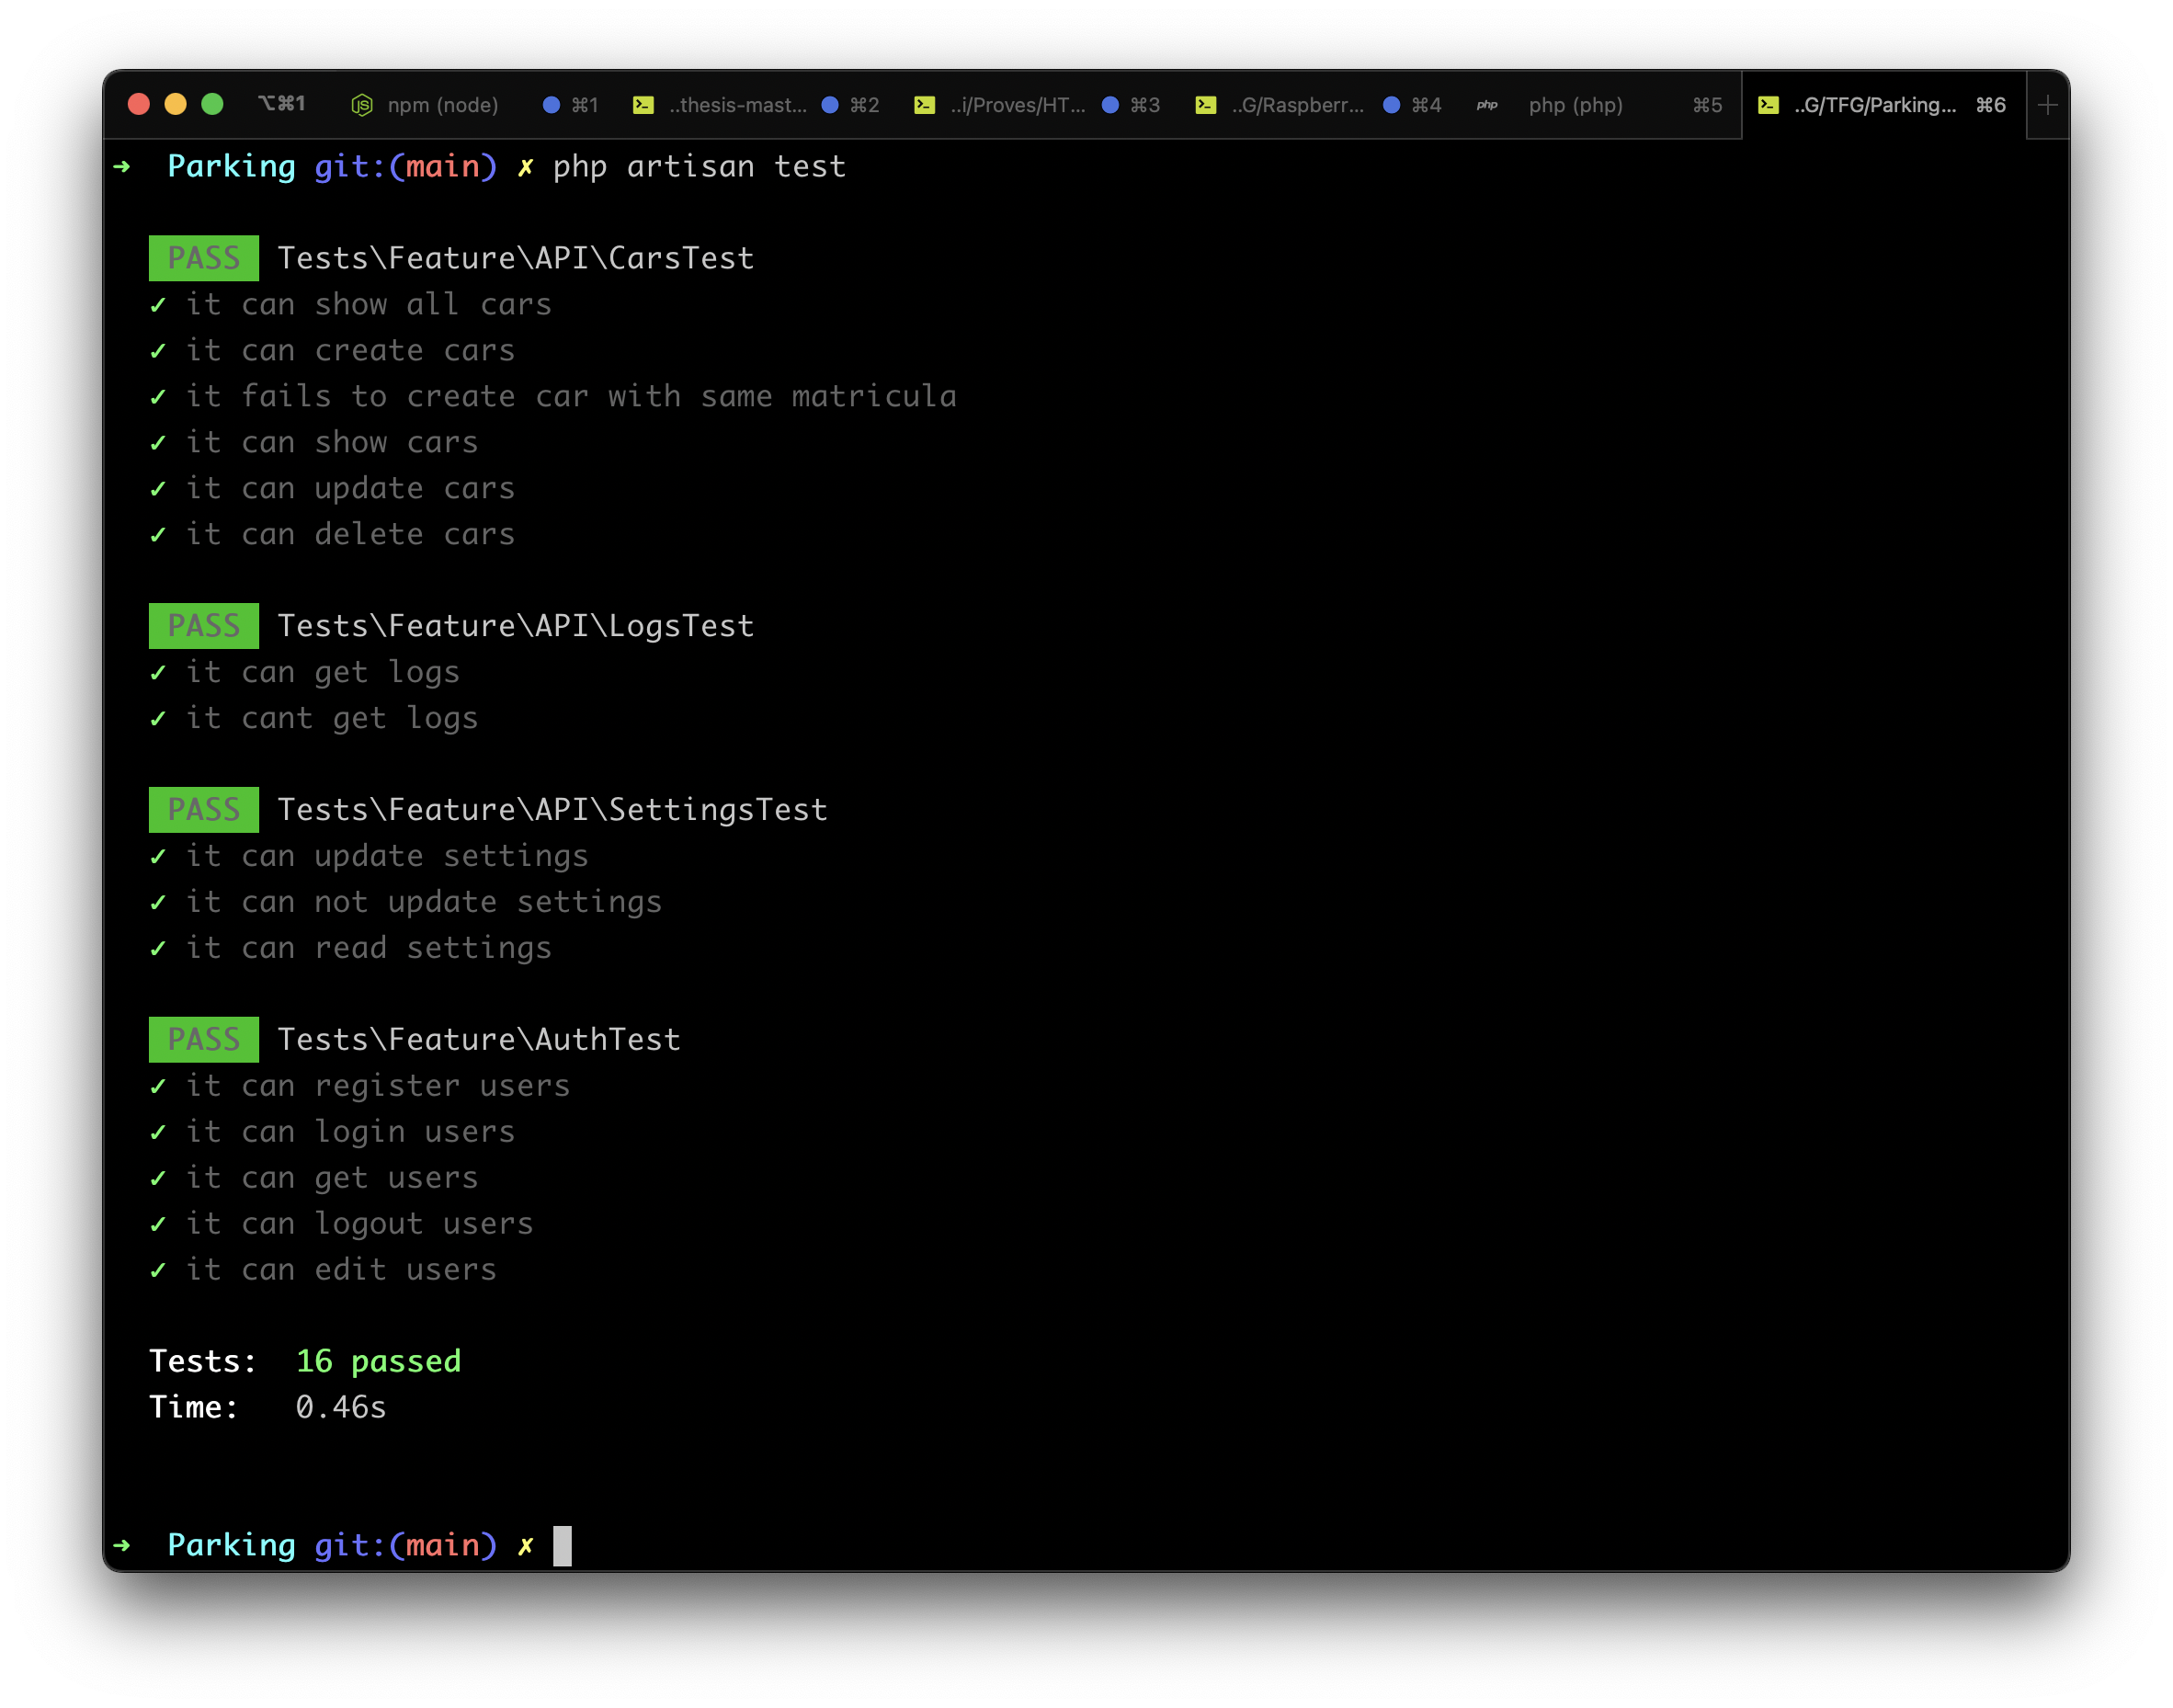
\includegraphics[scale=0.20]{Fotos/testsComprovacio.png}
    \end{center}
    \caption{Tests Correctes}
    \label{fig:register_photo}
\end{figure}

\chapter{Front-end}
La implementació del \emph{front-end} de l'aplicació, és a dir
la part que l'usuari interactua amb ella s'ha usat la \emph{framework} de \emph{NextJS}
\autocite{nextjs} basada en React.

\section{Elecció de l'entorn}

\emph{React}, és una llibreria de codi obert de JavaScript amb l'objectiu de desenvolupar interfícies d'usuari.
ReactJS permet als desenvolupadors crear aplicacions que fan servir dades que poden canviar
amb el temps sense la necessitat de recarregar la pàgina \autocite{react}. Les seves grans característiques
són la rapidesa, simplicitat i l'escalabilitat. Aquests objectius s'aconsegueixen gràcies a:

\begin{itemize}
    \item \emph{DOM Virtual} \emph{Document Object Model}: és el que permet renderitzar només
    els elements gràfics que han estat modificats, això aporta una gran velocitat. És
    útil quan es té moltes dades i hi ha petites modificacions.
    \item \emph{JSX}: és una extensió del llenguatge de programació JavaScript optimitzat
    en velocitat i captura errors en temps de compilació. L'usuari té la possibilitat
    d'utilitzar-la perquè ajuda al desenvolupador, ja que té una sintaxi semblant a la de
    l'HTML, això implica que fa el codi més llegible i escriure'l és una experiència
    similar a l'HTML, el fa més fàcil.
    \item Permet crear components reutilitzables.
\end{itemize}

Existeixen algunes \emph{frameworks} que usen la llibreria de \emph{React}, com per exemple,
\emph{NextJS} que fa servir tot el que dóna la llibreria de \emph{React}. A més, dóna un sistema
de rutes amb la separació de codi per ruta. Permet en la utilització d'eines que ajuden al
desenvolupador. Algunes d'elles utilitzades són:

\begin{itemize}
    \item \emph{Router}, per l'encaminament i la navegació.
    \item \emph{Link}, un component que permet que l'aplicació enllaci pàgines i carregui les
    seves dades.
\end{itemize}

El més a destacar és que permet la generació estàtica dels arxius, és a dir, precompila part
del codi que no és dinàmic.

\section{Pàgines}
En els annexos s'hi pot trobar un recull de fotografies per mostrar com és la part de \emph{front-end}.
Pel disseny de l'aplicació s'utilitza la \emph{framework} de CSS \texttt{Tailwind}. Usant
aquesta eina permet al desenvolupador evitar escriure arxius CSS \autocite{tailwind}.

\subsection{Iniciar Sessió}
En aquesta vista permet a l'usuari obrir la sessió posant el seu correu electrònic i la contrasenya
en els \emph{inputs} que es veuen a la imatge \autoref{fig:login_photo}. Seguidament, l'usuari ha
de prémer el botó d'\texttt{Iniciar sessió}. Si l'usuari no està registrat en aquesta aplicació, ho
 pot fer prement el botó de \emph{Crear un nou compte} que està sota del primer botó.

\subsection{Registrar usuari}
Aquesta vista mostra uns \emph{inputs} per incloure les dades de l'usuari per
poder-se registrar a l'aplicació. Aquests són el nom, el DNI, el telèfon mòbil, el correu electrònic, la contrasenya
i la confirmació de la contrasenya. Una vegada inscrites aquestes dades s'ha de prémer el botó de \emph{Registrar-se},
si es vol tirar enrere i anar a la pàgina d'iniciar sessió es pot clicar el botó de \emph{Ja tinc compte} o prémer el \emph{logo} de
la \emph{navbar}. La imatge relacionada aquesta vista es pot trobar a \autoref{fig:register_photo}.

\subsection{Principal}
La imatge que mostra un exemple d'aquesta vista està a \autoref{fig:index_photo}. En la fotografia es pot veure tres seccions.

La primera és que dóna la benvinguda a l'usuari i hi ha un botó que únicament es pot clicar quan està disponible.
La disponibilitat varia segons si l'usuari és administrador. La imatge corresponent a la part d'administradors
està a \autoref{fig:admin_photo}.

La segona, hi ha una \emph{card} on hi ha la informació de l'usuari, a la part superior a la dreta
hi ha una icona d'un llapis. Aquest llapis és un botó per editar aquesta informació. Quan l'usuari
el clica, l'aplicació redirigeix a l'usuari a una pantalla per editar-la. La pantalla d'editar està a
\autoref{fig:edit_user_photo}.

Finalment, es troba la tercera secció on també hi ha una \emph{card} on hi ha la informació dels vehicles
registrats de l'usuari. A la part superior d'aquesta \emph{card} hi ha un botó amb un \texttt{+},
si el client clica aquest botó, l'aplicació el redirigeix a una pantalla
per afegir vehicles, una imatge d'aquesta vista està a \autoref{fig:add_car_photo}.

Quan hi ha vehicles guardats es mostra el número de matrícula i tres botons. Aquests botons tenen tres
accions diferents, el primer canvia depenent d'on està el cotxe. Si el cotxe no està dins del pàrquing,
el botó és un codi QR, ja que per entrar al pàrquing s'ha de clicar. Es pot veure aquesta pantalla a
\autoref{fig:codiQR_photo}. En canvi, si el cotxe està dins del pàrquing la vista mostra una \texttt{P}
de pàrquing, on hi ha la informació relacionada d'aquest aparcament.
Un exemple d'aquesta pantalla és \autoref{fig:information_photo}.
El segon botó és un llapis, s'utilitza per editar el número de la matrícula.

La vista que controla aquesta funcionalitat és a \autoref{fig:edit_car_photo}. Per acabar, hi ha un botó
d'una brossa de color vermell. Aquest botó és per eliminar el vehicle.
Els botons d'editar i eliminar es deshabiliten quan el vehicle està estacionat dins del pàrquing.

\subsubsection{Vista per editar l'usuari}
En aquesta vista l'usuari pot modificar les dades del seu compte com el nom, la contrasenya, el telèfon i el DNI.
Es troben dos botons al final de la \emph{card} on el primer és per tirar enrere cap a la pantalla d'índex
\autoref{fig:index_photo}, també es pot anar a la pantalla principal clicant el \emph{logo} de la \emph{navbar}.
El segon botó és per guardar les noves dades a la base de dades. La imatge relacionada a aquesta vista és \autoref{fig:edit_user_photo}.

\subsubsection{Vista per editar els cotxes de l'usuari}
La imatge que mostra aquesta pantalla és \autoref{fig:edit_car_photo}. Es veu una \emph{card} on només hi ha un \emph{input}
per modificar el número de la matrícula.
El format pel número de la matrícula és \emph{xxxxXXX}, on els quatre primers caràcters són números del 0-9
i els tres caràcters del final són lletres de l'A-Z. La matrícula és única per cada usuari, és a dir, no es pot repetir.

\subsubsection{Vista per afegir els cotxes de l'usuari}
Aquesta vista és molt similar a l'anterior, ja que únicament canvia el títol i l'acció resultant,
és a dir afegir un cotxe a la base de dades amb l'usuari que ha iniciat sessió.
La següent imatge mostra aquesta vista \autoref{fig:add_car_photo}.

\subsection{Codi QR}
Quan l'usuari es troba a la pàgina principal i vol accedir amb un vehicle al pàrquing, clica el botó del codi QR que pertany en aquest vehicle.
Aquest botó redirigeix a aquesta pantalla \autoref{fig:codiQR_photo}. Es veu una \emph{card} on a dins hi ha el codi QR
generat per aquell vehicle. A sota d'aquest codi QR hi ha un botó, aquest botó serveix per generar un altre codi QR. Aquest botó
s'utilitza quan el codi QR generat no és vàlid
i es necessita crear-ne un altre per accedir dins del pàrquing.

A sota hi ha dos botons, el botó d'\emph{Enrere} per anar a la pantalla d'inici, també es pot usar el \emph{logo}
de la \emph{navbar} que redirigeix a la mateixa pàgina principal. A la dreta es pot veure un botó on diu \emph{Informació}
que s'activa quan el codi QR ha estat validat pel servidor i es pot entrar al pàrquing. En aquesta es veu la informació de l'estacionament.
Aquest botó, en principi no se'n fa ús, ja que el servidor envia un esdeveniment a l'aplicació a temps real i redirigeix
a la pàgina d'informació. Es pot veure un exemple a \autoref{fig:information_photo}.
Tot i això, aquest botó és útil per si hi ha algun problema que impedís l'enviament d'aquest esdeveniment.
D'aquesta manera l'aplicació es pot continuar fent servir.

\subsection{Informativa}
Aquesta pantalla ens mostra la informació de quina plaça té associada el cotxe, el dia i hora que ha entrat al pàrquing,
el preu en hora, la data actual i el preu en temps real. És una vista informativa. Quan es vol sortir del
pàrquing s'ha de prémer el botó de sortir que hi ha al final de la \emph{card} on es redirigeix a la pantalla
de pagament que es pot veure a \autoref{fig:payment_photo}. La següent imatge és un exemple del que pot mostrar aquesta pantalla
informativa \autoref{fig:information_photo}.

\subsection{Pagament}
Un cop s'ha pres el botó de sortir de la pantalla anterior es redirigeix a una pantalla de \emph{stripe}
per fer el pagament. Per simular un pagament amb èxit existeixen una llista de targetes
per fer \emph{testing}. Aquesta llista es pot trobar a \autocite{list_cards}.
Un exemple d'aquesta pantalla de pagament de \emph{Stripe} \autocite{stripe} està a \autoref{fig:payment_photo}.

\subsubsection{Pagament validat}
La pantalla de quan el pagament és validat consta d'un \emph{tick} de color verd
per mostrar que tot ha funcionat correctament. Un codi QR generat per sortir del pàrquing amb
un text explicatiu per saber que ha anat tot correctament i de quant temps es disposa
per la validesa d'aquest codi QR. Si aquests minuts s'accedeixen, s'ha de tornar a pagar.
Disposa d'un botó per anar a la pàgina principal, com també si es clica el \emph{logo} de la
\emph{navbar}. La vista es pot veure a \autoref{fig:payment_success_photo}.

\subsubsection{Pagament cence\l.lat}
En aquest cas, el pagament ha estat cance\l.lat per l'usuari. La vista és
una creu de color vermell que indica que hi ha hagut un error, a més una descripció posa que el pagament
no s'ha efectuat. Hi ha un botó per anar a la pàgina principal, com també si es clica el \emph{logo} de la
\emph{navbar}. La imatge d'aquesta vista es pot veure a \autoref{fig:payment_cancel_photo}

\subsection{Panell administració}
\label{sssec:index}
En aquest panell d'administració només hi pot accedir els usuaris que són \emph{admin}.
Els altres usuaris no hi poden accedir i a més tenen el botó deshabilitat.
Com es pot observar en la imatge d'aquesta vista a \autoref{fig:admin_photo} hi ha
dues \emph{cards}. La primera l'administrador pot modificar el preu en hores del
pàrquing, s'ha de posar en cèntims i també pot modificar el temps de validesa dels
codis QR. La segona hi ha una taula on es mostren tots els \emph{logs}, és a dir, totes
les entrades, sortides i pagaments efectuats al pàrquing. A la columna de \emph{pagament}
hi ha un enllaç cap a \emph{stripe} on hi ha la informació del pagament.
En aquesta pantalla es pot fer accions com descarregar les factures, tramitar devolucions,
veure detalls de la transacció i client \autocite{stripe}.
La imatge es pot veure a \autoref{fig:stripe_info_photo}.

\section{Eines utilitzades}

En aquesta aplicació es fan servir diferents eines importants per fer un correcte funcionament.
Aquestes eines són:

\begin{itemize}
    \item \texttt{Axios} \autocite{axios}: Aquesta eina permet fer peticions HTTP passant-li en els \emph{Authoritzon Header} el \emph{Barear Token} de l'usuari.
    El fet aquest es pot configurar de manera automàtica si s'activa les \emph{withCredentials} d'axios o es pot passar manual.
    \item \texttt{classnames} \autocite{classnames}: Una senzilla utilitat de JavaScript per unir condicionalment classNames.
    \item \texttt{dayjs} \autocite{dayjs}: Una llibreria de JavaScript de manipulació de dates.
    \item \texttt{pusher-js} \autocite{pusher}: Els canals de Pusher són una solució als \emph{Web Sockets}.
    Eina útil per crear aplicacions interactives en temps real.
    \item \texttt{react-qr-codes} \autocite{react_qr_code}: Un component de React per crear codis QR.
    \item \texttt{swr} \autocite{swr}: Utilitat que permet evitar peticions HTTP innecessàries utilitzant una \emph{cache}.
\end{itemize}


\chapter{Raspberry Pi}
\label{chap:raspberryPi}

La part de la barrera del pàrquing està composta per una Raspberry Pi 4 model B,
una càmera HQ, un LED RGB que simbolitzen les accions de la barrera, tres resistències de 470 Ohms
per fer les connexions amb el LED i per últim un brunzidor elèctric.


\subsection{Connexions}
Aquests components han d'estar connectats a la Raspberry Pi,
seguidament es mostra en els pins que s'han connectat cada un dels LEDs
i el brunzidor. Adjuntant un esquema dels pins de la Raspberry Pi per veure
quins són:

\begin{itemize}
    \item LED Red: GPIO 18
    \item LED Blue: GPIO 23
    \item LED Green: GPIO 24
    \item Brunzidor: GPIO 25
\end{itemize}

\begin{figure}[H]
    \begin{center}
        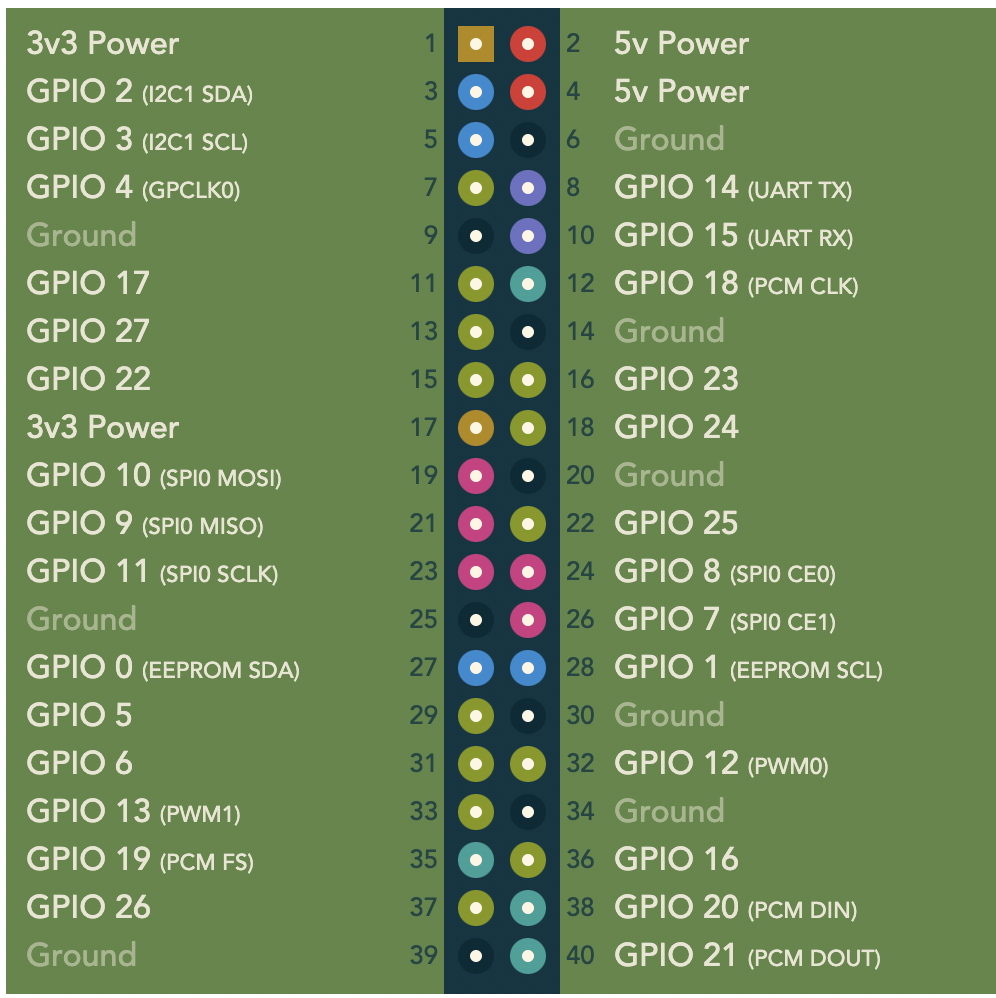
\includegraphics[scale=0.35]{Fotos/rasp_pinout.png}
    \end{center}
    \caption{Raspberry PI 4 pinout}
    \label{fig:payment_photo}
\end{figure}

Finalment, tots els components utilitzats amb el seu muntatge són els següents:

\begin{figure}[H]
    \begin{center}
        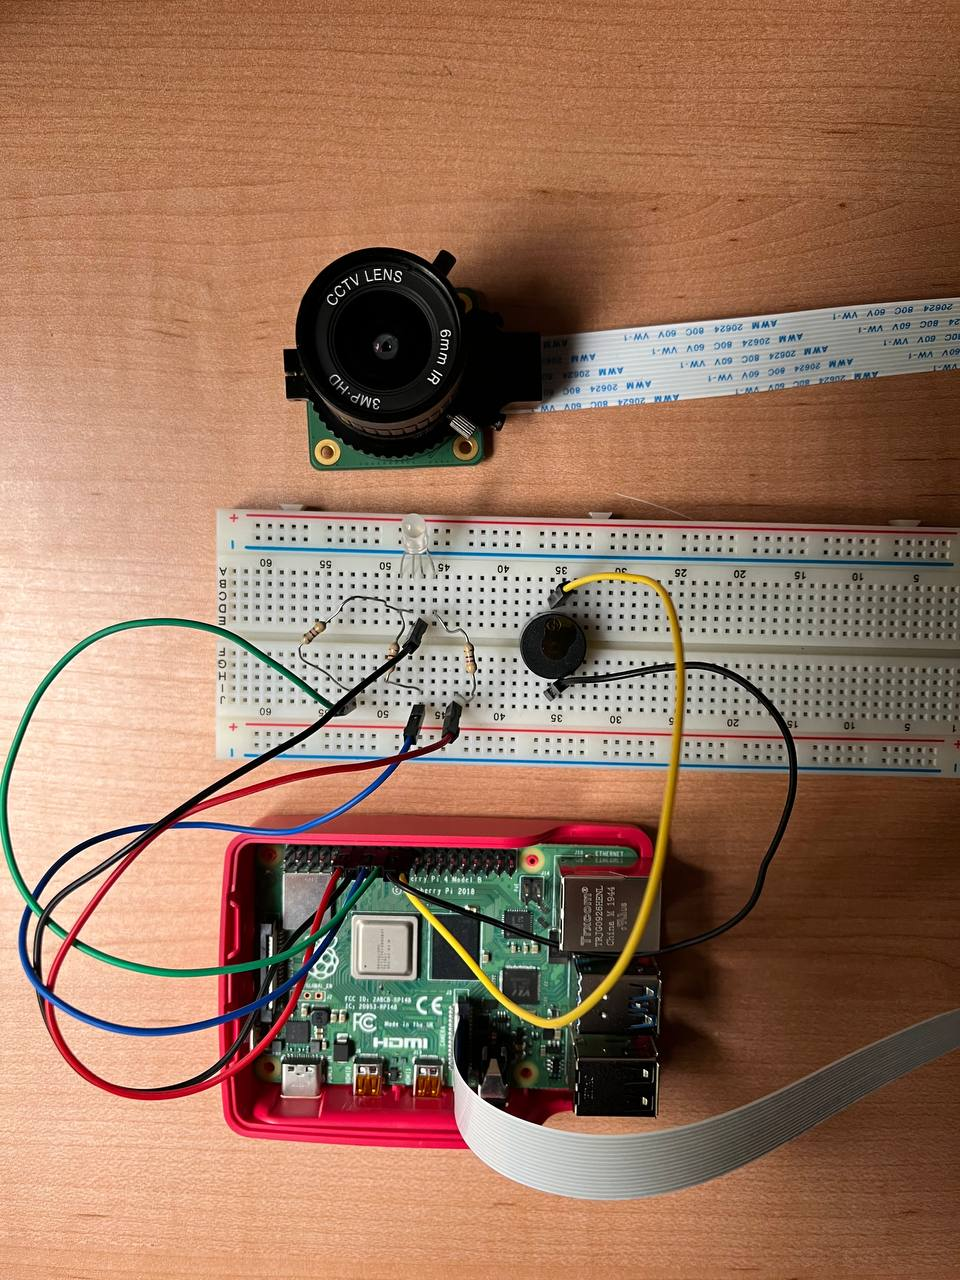
\includegraphics[scale=0.28]{Fotos/material.jpeg}
    \end{center}
    \caption{Muntatge Raspberry Pi}
    \label{fig:material}
\end{figure}


\subsection{Màquina d'estats}

\begin{figure}[H]
\begin{center}
    \includegraphics[scale=0.15]{Fotos/barrera.png}
\end{center}
\caption{Màquina d'estat detecció codi QR}
\label{fig:maq_estats}
\end{figure}

\begin{enumerate}
    \item \texttt{Estat 0}: Indica que la barrera està baixada posant el LED de color vermell a \emph{ON}.
    Obra la càmera connectada a la Raspberry Pi on es prepara per detectar codis QR.
    Quan en detecta un llegeix el seu contingut i el guarda a la variable anomenada
    \emph{qr}.
    Deshabilita la càmera, d'aquesta manera no pot detectar més codis QR.
    Quan detecta el codi QR s'activa el brunzidor que dura cinc segons i canvia al següent estat, l'estat 1.
    \item \texttt{Estat 1}: Es deshabilita el brunzidor. Apaga el LED vermell i posa a \emph{ON} el LED blau, ja
    que aquest LED indica que està fent la petició HTTP. Es guarda la resposta d'aquesta petició
    a una variable anomenada \emph{respostaHTTP}. Canvia al següent estat, l'estat 2.
    \item \texttt{Estat 2}: Apaga el LED blau, i comprova la resposta HTTP. Si la resposta
    és \texttt{204}, canvia l'estat a Estat 4. Si no ho és, canvia l'estat a l'estat 3.
    \item \texttt{Estat 3}: Per indicar a l'usuari que la resposta no ha sigut
    satisfactòria, el LED vermell farà quatre pampallugues.
    Finalment, l'estat passa a ser l'estat inicial, l'estat 0.
    \item \texttt{Estat 4}: Aquest estat és quan la resposta HTTP ha sigut satisfactòria.
    En aquest estat el LED Verd farà quatre pampallugues indicant que la barrera està pujant.
    Quan la barrera ha pujat, l'estat passa a ser l'estat 5.
    \item \texttt{Estat 5}: Posa el LED verd a \emph{ON}. Simbolitza la barrera pujada.
    Quan ha passat el temps corresponent canvia l'estat a l'estat 6.
    \item \texttt{Estat 6}: Aquest estat es comporta igual que l'estat 4. El LED Verd
    fa quatre pampallugues per indicar que la barrera està baixant.
    Quan es troba a abaixada passa a l'estat inicial. L'estat 0.
\end{enumerate}


\subsubsection{Llibreries}
Les llibreries utilitzades per fer la màquina d'estats anteriors
són les següents:
\begin{itemize}
    \item Requests: per fer peticions HTTP \autocite{requests}.
    \item Enum: Per declarar els estats \autocite{enum_python}. Tot i que aquesta llibreria
    és de la llibreria estàndard de Python.
    \item Time: Per fer la durada. S'utilitza la funció \emph{sleep()}. Tot i que aquesta llibreria
    és de la llibreria estàndard de Python.
    Com que el codi no fa res més no passa res que sigui bloquejant \autocite{sleep_python}
    \item RPi.GPIO: Per configurar els inputs de la Raspberry Pi \autocite{gpio_rasp}.
    \item cv2: Per obrir la càmera \autocite{cv2}.
    \item Pyzbar: Detectar codis QR, llegir-los i descodificar-los \autocite{pyzbar}.
\end{itemize}



\chapter{Connexions de hardware}
El projecte està compost per tres conjunts, el servidor de Laravel,
l'aplicació amb què l'usuari interactua i la barrera.
Pel desenvolupament d'aquest projecte s'ha organitzat de la manera que
el servidor i l'aplicació estan a un ordinador i la barrera està en una Raspberry Pi.

L'esquema que mostra com s'ha treballat durant el seu desenvolupament
és el següent:

\begin{figure}[H]
    \begin{center}
        \includegraphics[scale=0.28]{Fotos/connexióRasp-pc-mobile.png}
    \end{center}
    \caption{Connexions dels dispositius}
    \label{fig:material}
\end{figure}

\begin{itemize}
    \item El telèfon mòbil crea un punt d'accés personal.
    \item La Raspberry Pi i l'ordinador estan connectats a través d'un cable
    Ethernet.
    \item La Raspberry Pi està connectada al punt d'accés personal del telèfon mòbil
    i proporciona internet a l'ordinador.
\end{itemize}

Per poder aconseguir aquesta configuració a la barrera, concretament a la Raspberry Pi, se li ha assignat una
adreça IP a \texttt{eth0}, la qual és 10.10.10.10.
A l'ordinador, es configura l'adreça 10.10.10.1 amb l'encaminador 10.10.10.10.
D'aquesta manera hi ha la possibilitat de connectar-se amb la Raspberry Pi
via \texttt{ssh} fent \texttt{ssh pi@10.10.10.10} des d'un terminal de l'ordinador.
D'aquesta manera es pot utilitzar la Raspberry Pi des del mateix ordinador
sense la necessitat de connectar una pantalla externa i perifèrics com el ratolí
i el teclat. Tot i que al principi s'accedia a la Raspberry Pi a través d'una pantalla
per tal de configurar la càmera i fer les configuracions anteriors de l'esquema \autoref{fig:material}.

Pel projecte es necessita que la barrera tingui connexió a internet, ja que
fa peticions HTTP. També es vol que el servidor i l'aplicació tinguin internet,
perquè si no no es poden fer ús dels esdeveniments de \texttt{WebSockets} que utilitzen
i altres eines o llibreries que se'n fa ús.

La solució d'aquest problema que es planteja és
configurar la Raspberry Pi de tal manera que l'ordinador tingui accés a internet a través d'ella,
ja que és qui li proporciona internet des de la \emph{wlan0}.
S'ha d'activar l'\texttt{ip forwarding} de la Raspberry Pi, d'aquesta manera ella pot actuar
com a \textsl{router}.

Per aconseguir aquest efecte es fa servir la comanda següent:
\texttt{iptables -t nat -A POSTROUTING -s 10.10.10.0/24 -o wlan0 -j MASQUERADE}.
Per fer això persistent i no posar la comanda cada vegada que es vol
provar el funcionament del projecte cal modificar el fitxer d'\emph{/etc/iptables/rules.v4}
posant la comanda següent a l'apartat de \emph{nat}:

\texttt{-A POSTROUTING -s 10.10.10.0/24 -o wlan0 -j MASQUERADE}


Aquesta comanda és afegir a la taula \texttt{nat} la regla \emph{POSTROUTING},
aquesta regla consisteix a alterar o fer una determinada acció als paquets quan estan a punt de sortir
on la font és l'adreça 10.10.10.0/24 i s'envien els paquets a través de
la interfície \texttt{wlan0} cap a l'objectiu \emph{MASQUERADE}.
Aquesta, s'utilitza per IP dinàmiques, la qual el telèfon mòbil equival a una d'elles.
Per més informació d'aquesta comanda es pot trobar a \autocite{man_iptables}.
A més, configurar un servidor DNS a l'ordinador, el DNS 8.8.8.8.

\chapter{Desglossament econòmic de la demo}

\begin{table}[H]
\centering
\begin{tabular}{llll}
\hline
    \textbf{Nom} & \textbf{Quantitat} & \textbf{Preu} \\ \hline
    RASPBERRY PI 4 MODEL B 4GB & 1 & 59,95 € \\ \hline
    CAMARA HQ OFICIAL RASPBERRY PI & 1 & 55,95 € \\ \hline
    CAJA OFICIAL RASPBERRY PI 4 & 1 & 6,95 € \\ \hline
    CABLE MICRO HDMI 1M. \\ NEGRE OFICIAL RASPBERRY PI & 1 & 5,95 € \\ \hline
    SOFTWARE NOOBS PREINSTA\L.LAT \\ EN MICROSD 16GB \\ PARA RASPBERRY PI & 1 & 7,95 € \\ \hline
    LENT FIXA 6MM MUNTURA CS & 1 & 28,95 € \\ \hline
    \textbf{TOTAL} & \textbf{6} & \textbf{165,7€} \\ \hline
\end{tabular}
\caption{Preus material necessari per a la demostració}
\label{tab:my-pressupost}
\end{table}

En aquest desglossament s'ha de tenir en compte el preu del lloguer del servidor.

\section{Material necessari per barrera}

\begin{itemize}
    \item Placa Raspberry Pi 4 4GB \autocite{raspberry_Pi}.
    \item Raspberry Pi High Quality Camera \autocite{camera_rasp}.
    \item Lent fixa 6mm monturs CS \autocite{lent_rpi}.
    \item LED RGB (tret del laboratori de DIPSE).
    \item Tres resistències de 470 Ohms (tret del laboratori de DIPSE).
    \item Brunzidor (tret del laboratori de DIPSE).
\end{itemize}

\chapter{Conclusions}
Pel que fa a la realització d'aquest TFG, s'ha assolit el propòsit principal
que és realitzar una aplicació (una \emph{demo}) per la gestió automatitzada d'un pàrquing
inte\l.ligent amb el seu control d'entrades i sortides, amb la part de pagament i un panell administratiu.

Per dur a terme aquest projecte s'ha trobat algunes dificultats, les quals són:

Primer de tot, amb la part de \emph{back-end}:
\begin{itemize}
    \item Crear la composició del codi QR i buscar la forma de què aquests codis siguin vàlids.
    \item Com ha d'actuar el servidor quan rep la lectura d'un codi QR i les accions que ha de
    prendre respecte si és vàlid o no.
    \item En el sistema de pagament, la dificultat és passar-li \emph{metadata} per
    obtenir la informació de qui havia fet el pagament evitant passar les dades per l'URL. D'aquesta manera s'evita que
    l'usuari pugui modificar-la.
    \item Decidir com associar les places als usuaris, és a dir de donar la possibilitat a l'usuari a escollir la plaça
    desitjada o que l'aplicació faci aquesta assignació.
\end{itemize}

Per l'apartat de \emph{front-end} la utilització dels \emph{hooks} que disposa la llibreria
de \emph{React}. Aquests són el \emph{UseCallback}, \emph{useMemo}, \emph{useState} i el \emph{useContext}.
L'explicació d'aquestes eines es poden trobar a \autocite{hooks_react}.

Finalment, per l'apartat de la \emph{Raspberry Pi}:
\begin{itemize}
    \item Buscar eines o llibreries per obrir la càmera de la Raspberry pi.
    \item Buscar llibreries per la detecció als codis QR i la lectura d'aquests.
    \item Buscar una eina per fer peticions HTTP.
    \item Realitzar una màquina d'estats més robusta i que contempli possibles casos d'error, com el d'invalidesa del codi QR.
    \item Buscar components electrònics per tal de poder fer una simulació d'una barrera de pàrquing.
\end{itemize}

Finalment, treballar totes aquestes aplicacions conjuntament i poder fer una demostració de la seva funcionalitat
ha comportat problemes, a causa de la necessitat de controlar la Raspberry Pi per \emph{ssh} i que tots dos conjunts obtinguessin internet.

\section{Treball futur}

Com a treball futur es proposen algunes millores al projecte per tal d'assolir més funcionalitats:

\begin{enumerate}
    \item Afegir o crear un control per part d'administració que pugui pujar o baixar
    la barrera depenent de les necessitats o problemes que puguin succeir. Exceptuant una
    fallada de motor. Per aconseguir aquest efecte és fer que l'actual servidor,
    és a dir, \emph{Laravel} (o \emph{back-end}), passi a ser un client i la Raspberry Pi passi a ser
    un servidor de \emph{Python}. Fer una connexió bidireccional.
    A més a més, crear una taula a la base de dades on es guarda la \emph{ID} i l'estat de la barrera.
    \item Afegir un espai on els usuaris puguin canviar la plaça assignada i puguin
    escollir la plaça desitjada. En l'aplicació fer que els usuaris vegin un mapa
    del pàrquing on pugui seleccionar la plaça, on també mostra les places ocupades
    i lliures en temps real.
    \item Posar la possibilitat de fer reserves de places a través de l'aplicació.
    \item Fins ara, el control d'entrades, sortides i pagaments la veuen els administradors.
    Afegir una pantalla on els clients puguin veure aquesta informació i descarregar-se la factura.
    \item Configurar el servidor de \emph{Laravel} per enviar correus als clients adjuntant la factura
    de cada pagament.
\end{enumerate}




\chapter{Bibliografia}
\printbibliography[heading=none]

% % Capitols appendix
\part{Annexos}

\appendix

\chapter{Images del front-end de l'aplicació}
\begin{figure}[H]
    \begin{center}
        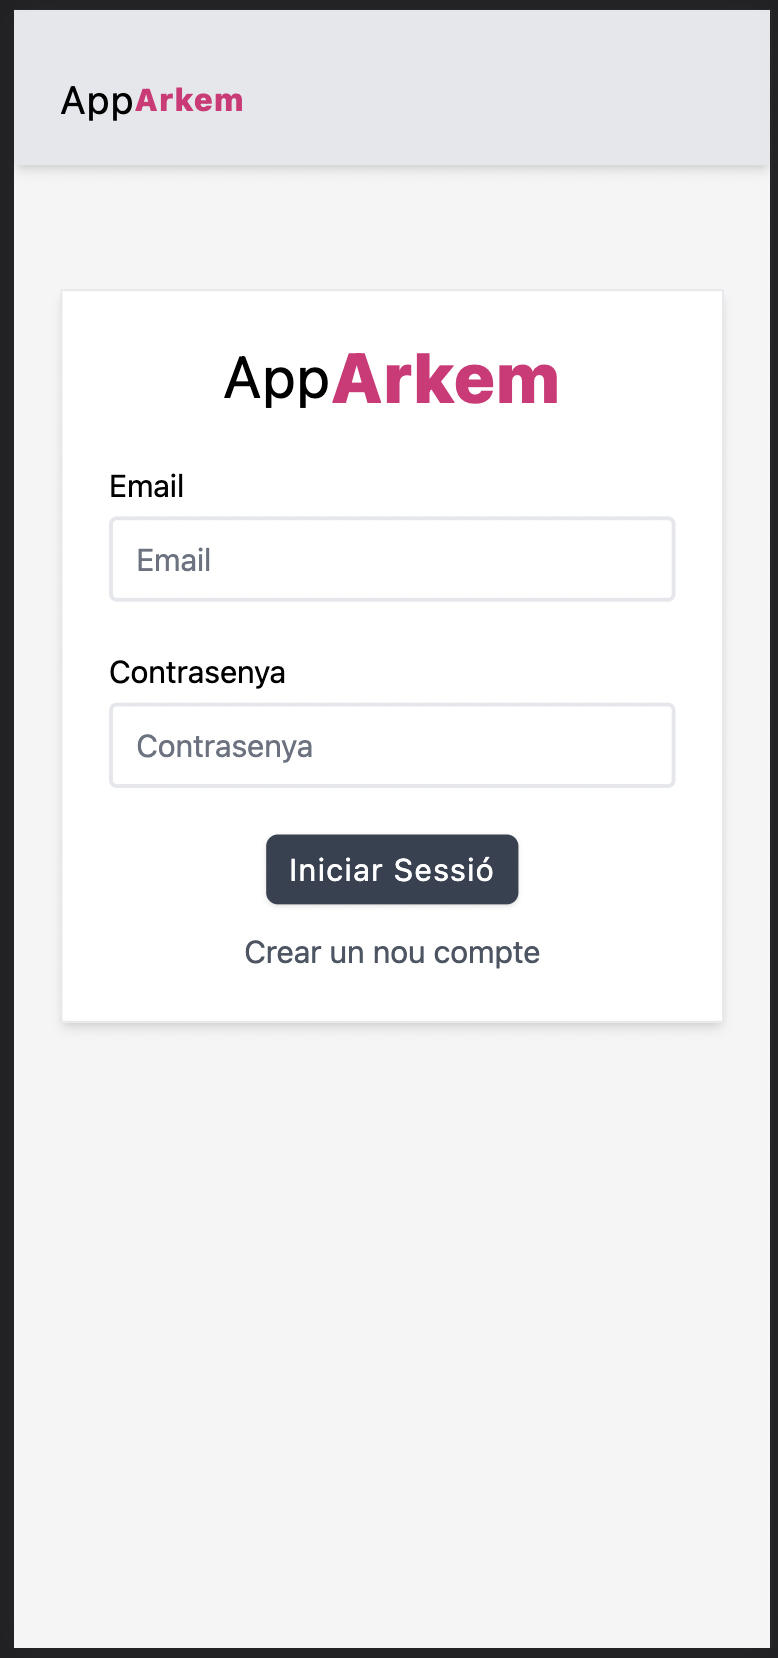
\includegraphics[scale=0.50]{Fotos/pantalla0_login.png}
    \end{center}
    \caption{Pantalla d'iniciar sessió}
    \label{fig:login_photo}
\end{figure}

\begin{figure}[H]
    \begin{center}
        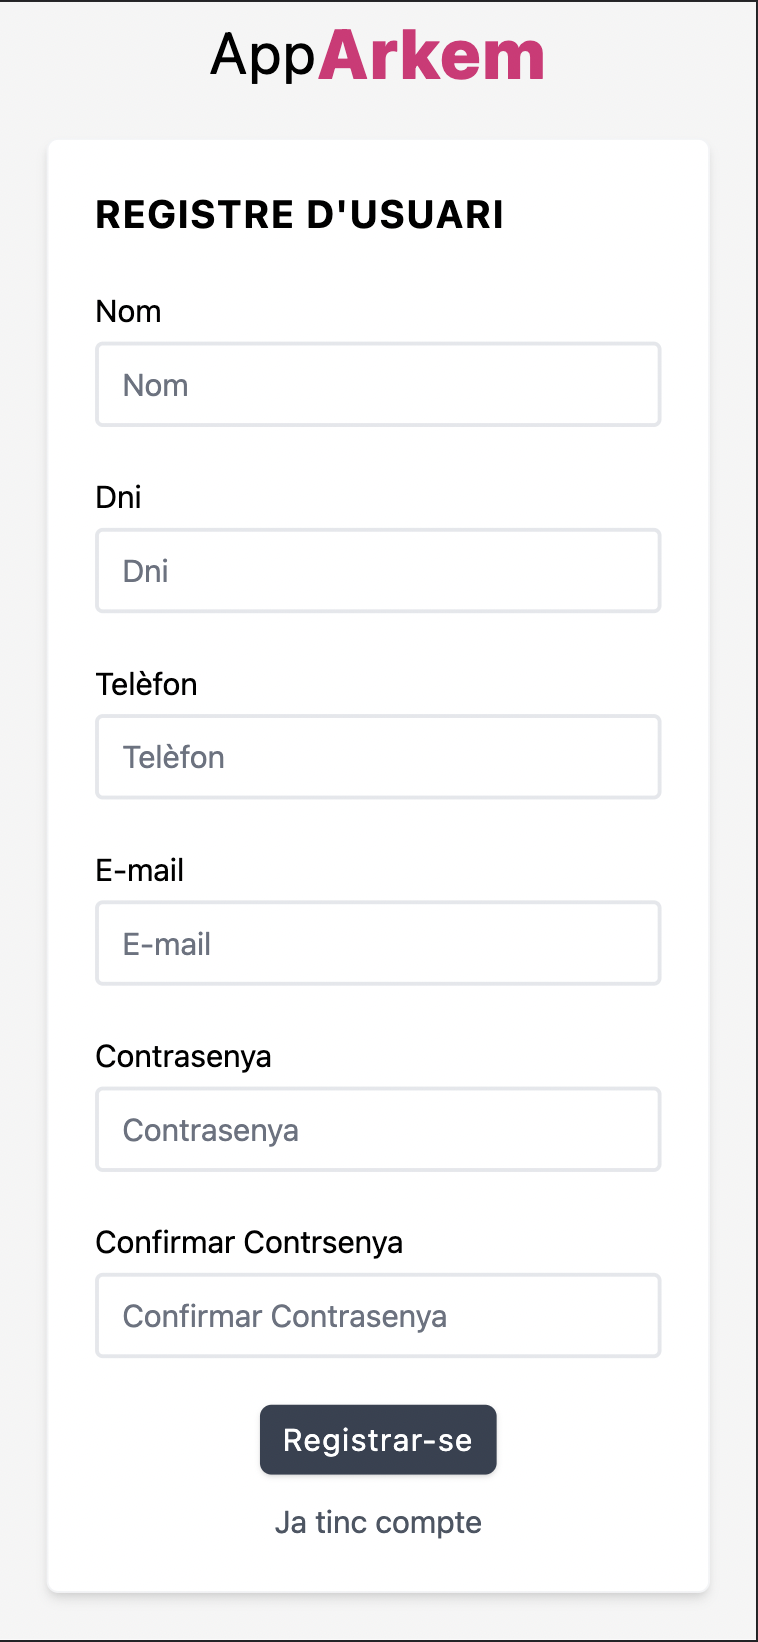
\includegraphics[scale=0.50]{Fotos/pantalla1_registre.png}
    \end{center}
    \caption{Pantalla de registrar usuaris}
    \label{fig:register_photo}
\end{figure}

\begin{figure}[H]
    \begin{center}
        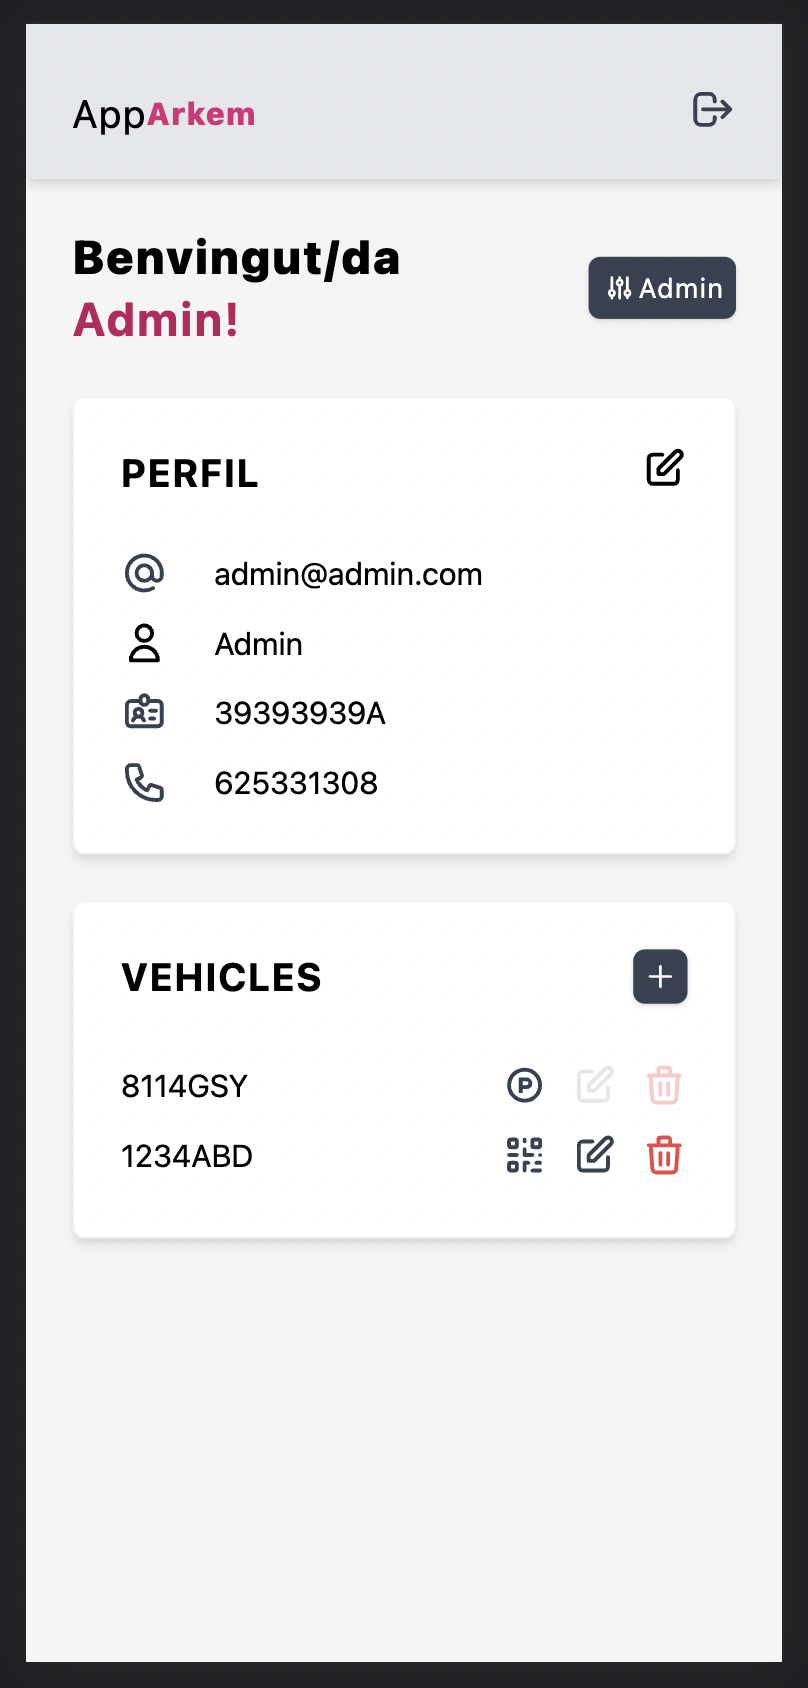
\includegraphics[scale=0.50]{Fotos/pantalla2_index.png}
    \end{center}
    \caption{Pantalla principal}
    \label{fig:index_photo}
\end{figure}

\begin{figure}[H]
    \begin{center}
        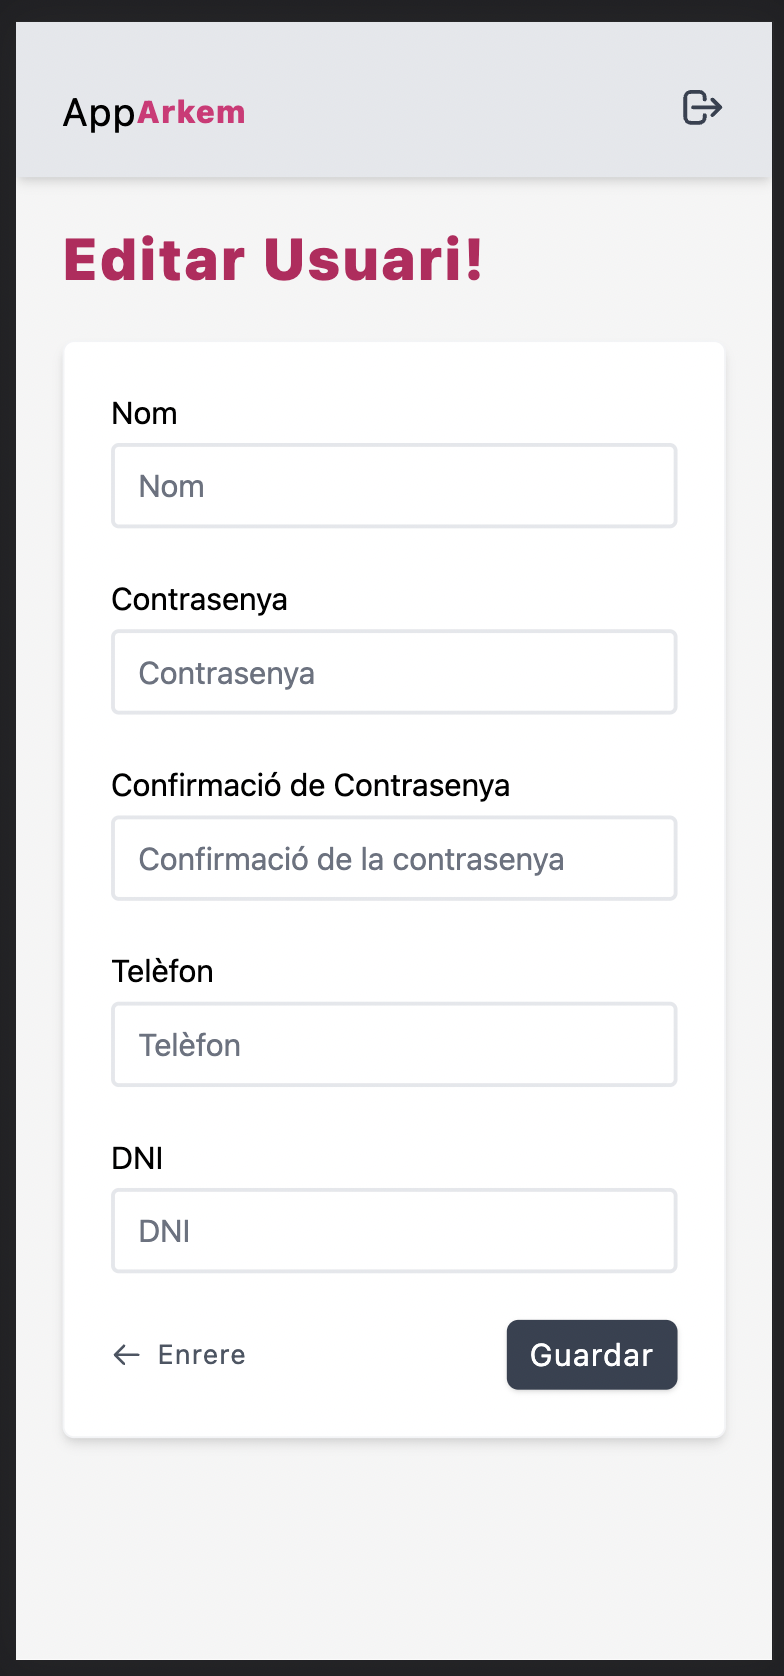
\includegraphics[scale=0.50]{Fotos/pantalla9_edit_user.png}
    \end{center}
    \caption{Pantalla d'editar informació de l'usuari}
    \label{fig:edit_user_photo}
\end{figure}

\begin{figure}[H]
    \begin{center}
        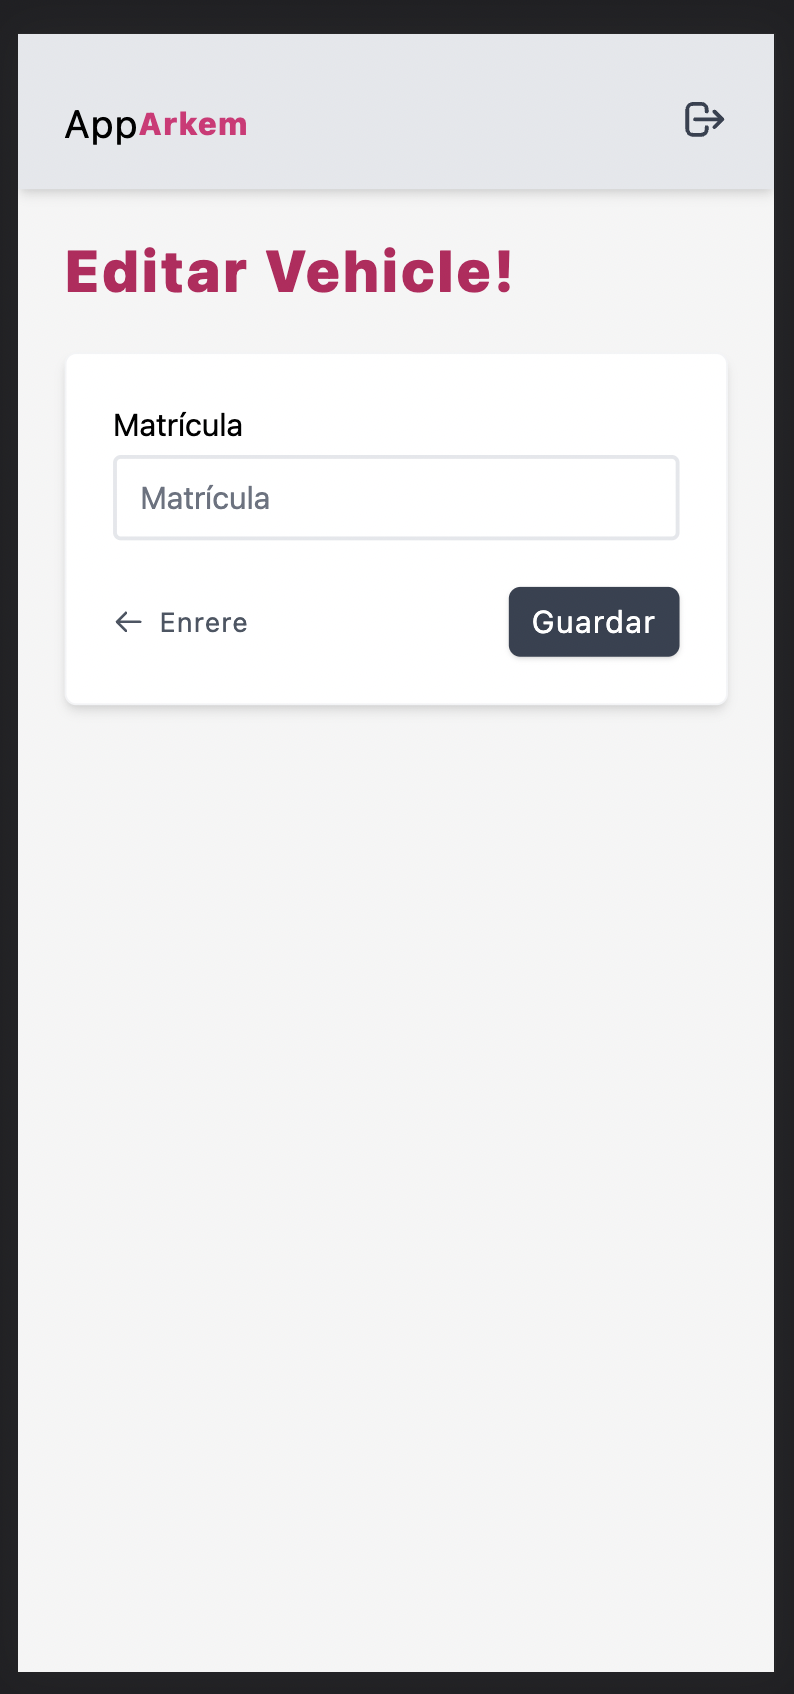
\includegraphics[scale=0.50]{Fotos/pantalla10_edit_car.png}
    \end{center}
    \caption{Pantalla editar cotxes de l'usuari}
    \label{fig:edit_car_photo}
\end{figure}

\begin{figure}[H]
    \begin{center}
        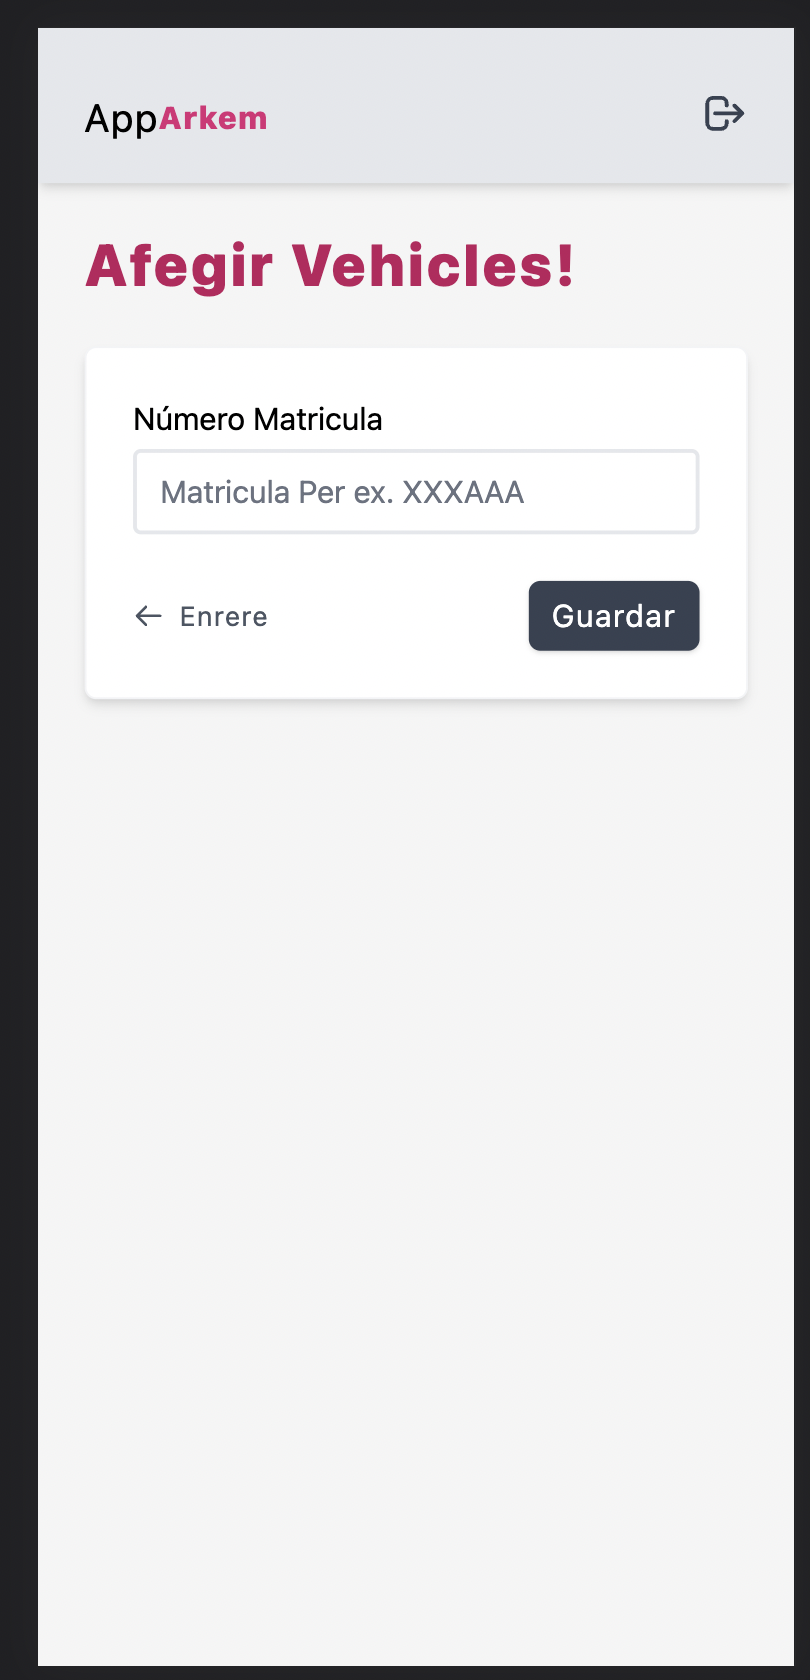
\includegraphics[scale=0.50]{Fotos/pantalla11_add_car.png}
    \end{center}
    \caption{Pantalla d'afegir cotxes de l'usuari}
    \label{fig:add_car_photo}
\end{figure}

\begin{figure}[H]
    \begin{center}
        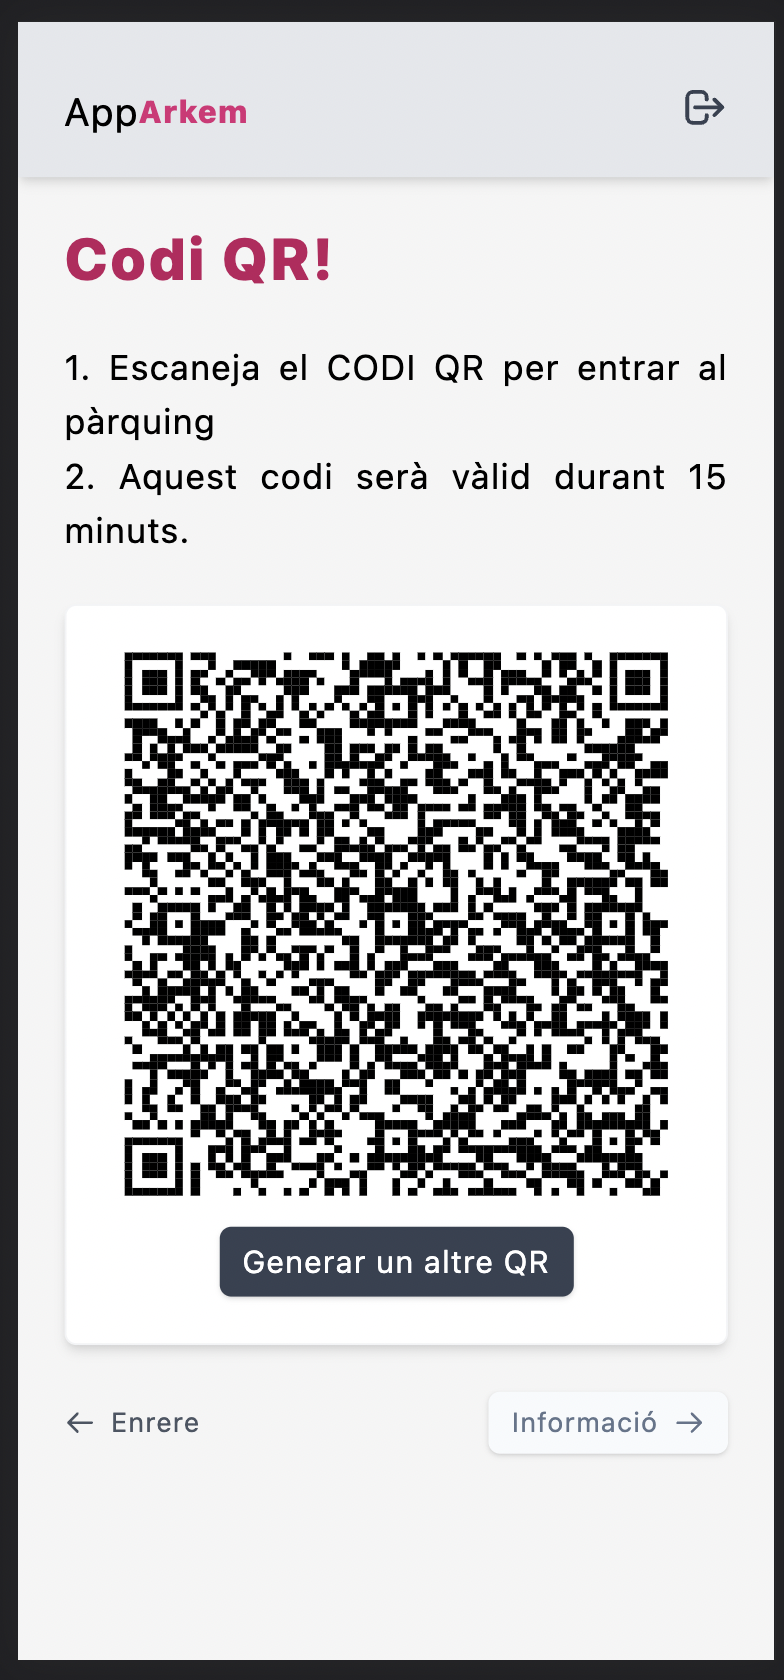
\includegraphics[scale=0.50]{Fotos/pantalla3_codiQR.png}
    \end{center}
    \caption{Pantalla generar codi QR}
    \label{fig:codiQR_photo}
\end{figure}

\begin{figure}[H]
    \begin{center}
        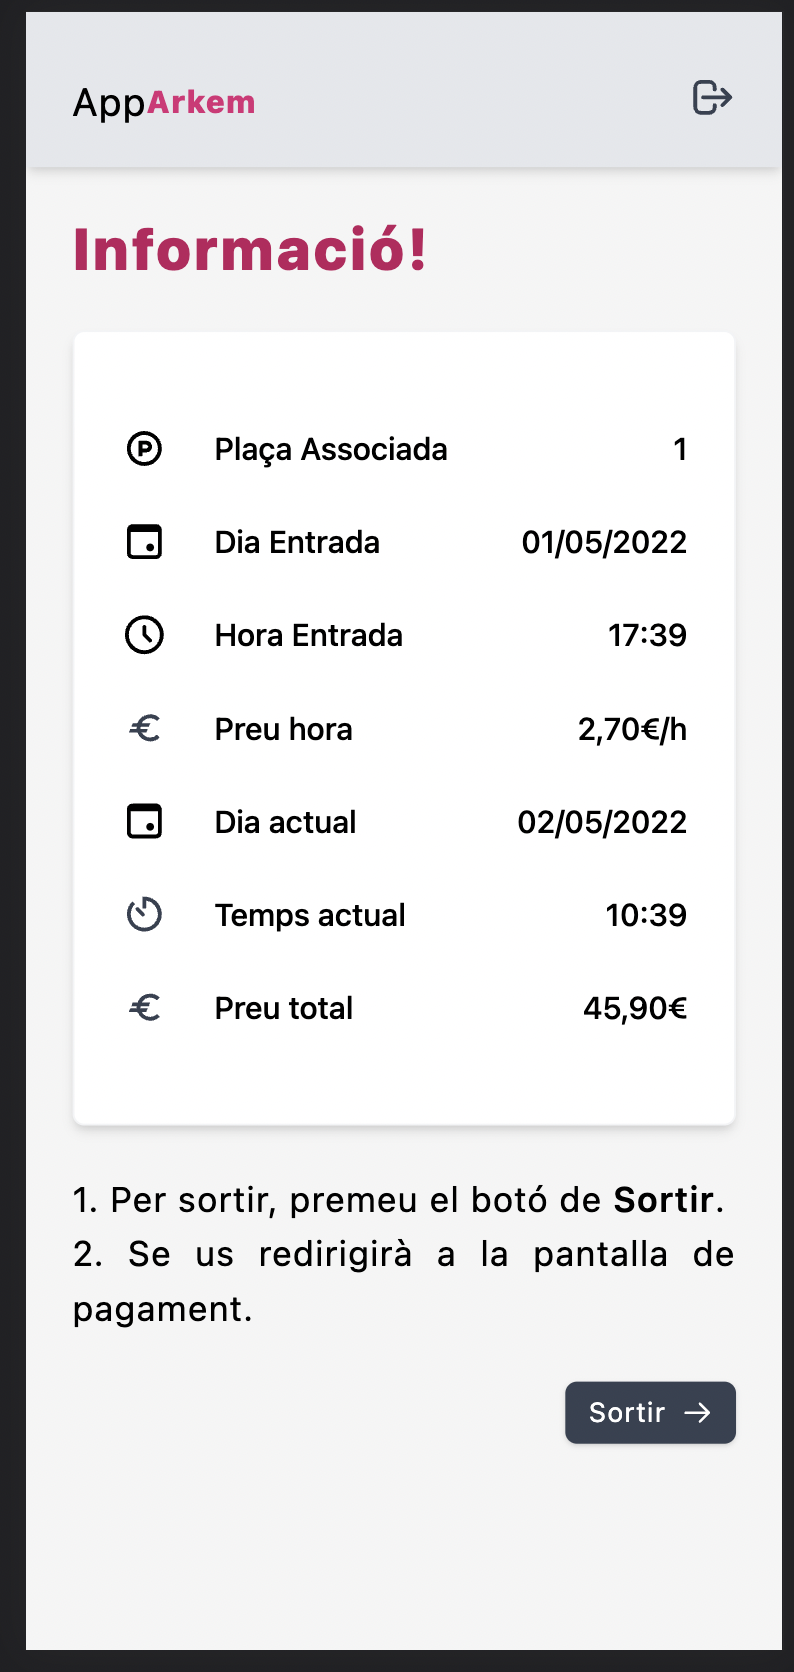
\includegraphics[scale=0.50]{Fotos/pantalla4_informacio.png}
    \end{center}
    \caption{Pantalla d'informació de l'aparcament}
    \label{fig:information_photo}
\end{figure}

\begin{figure}[H]
    \begin{center}
        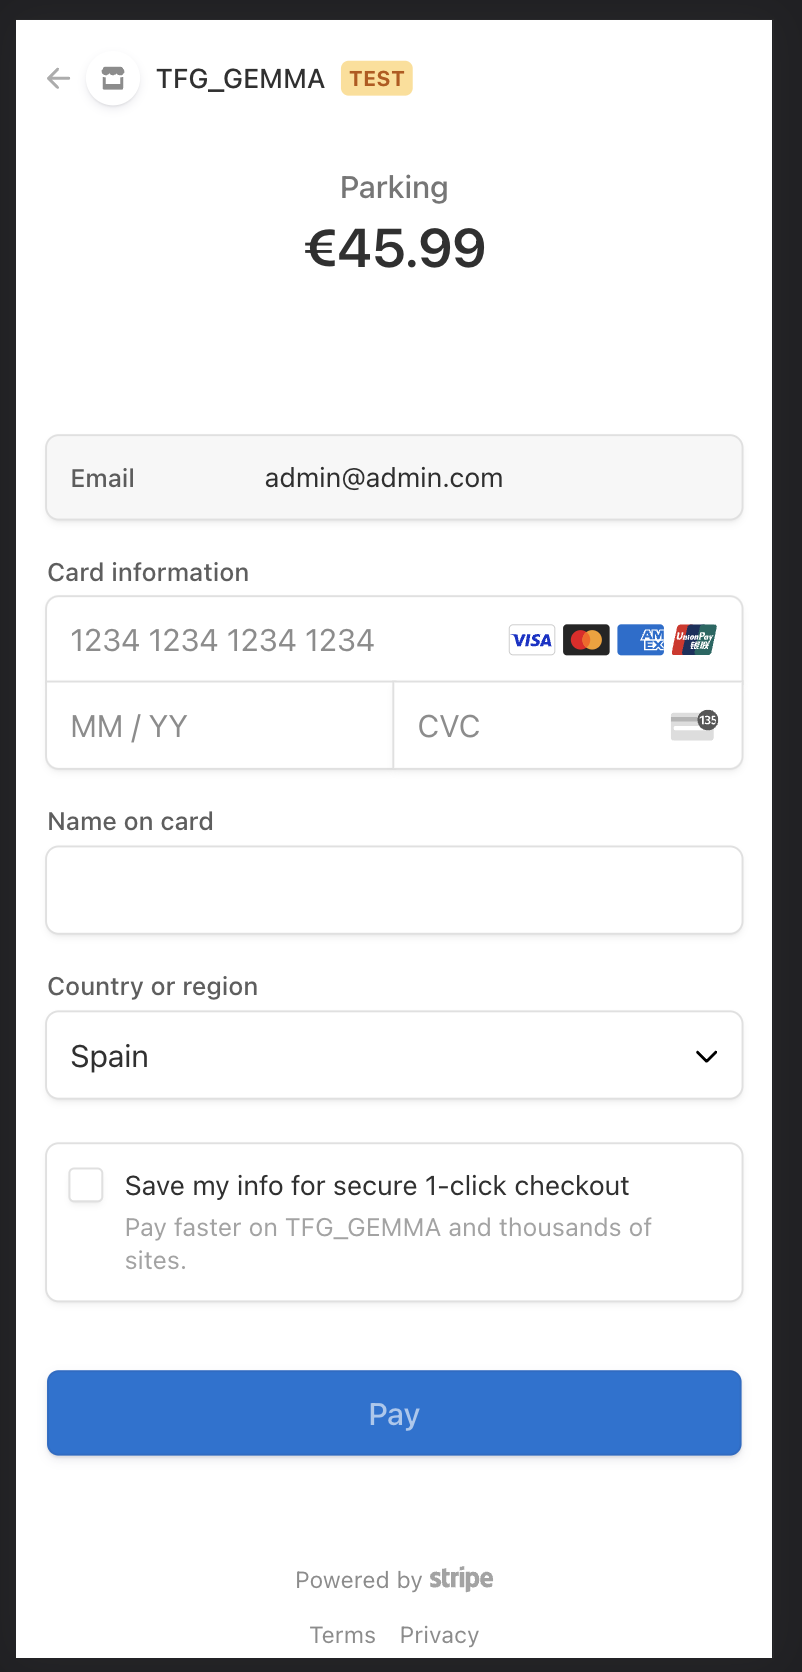
\includegraphics[scale=0.50]{Fotos/pantalla5_pagament.png}
    \end{center}
    \caption{Pantalla del pagament}
    \label{fig:payment_photo}
\end{figure}

\begin{figure}[H]
    \begin{center}
        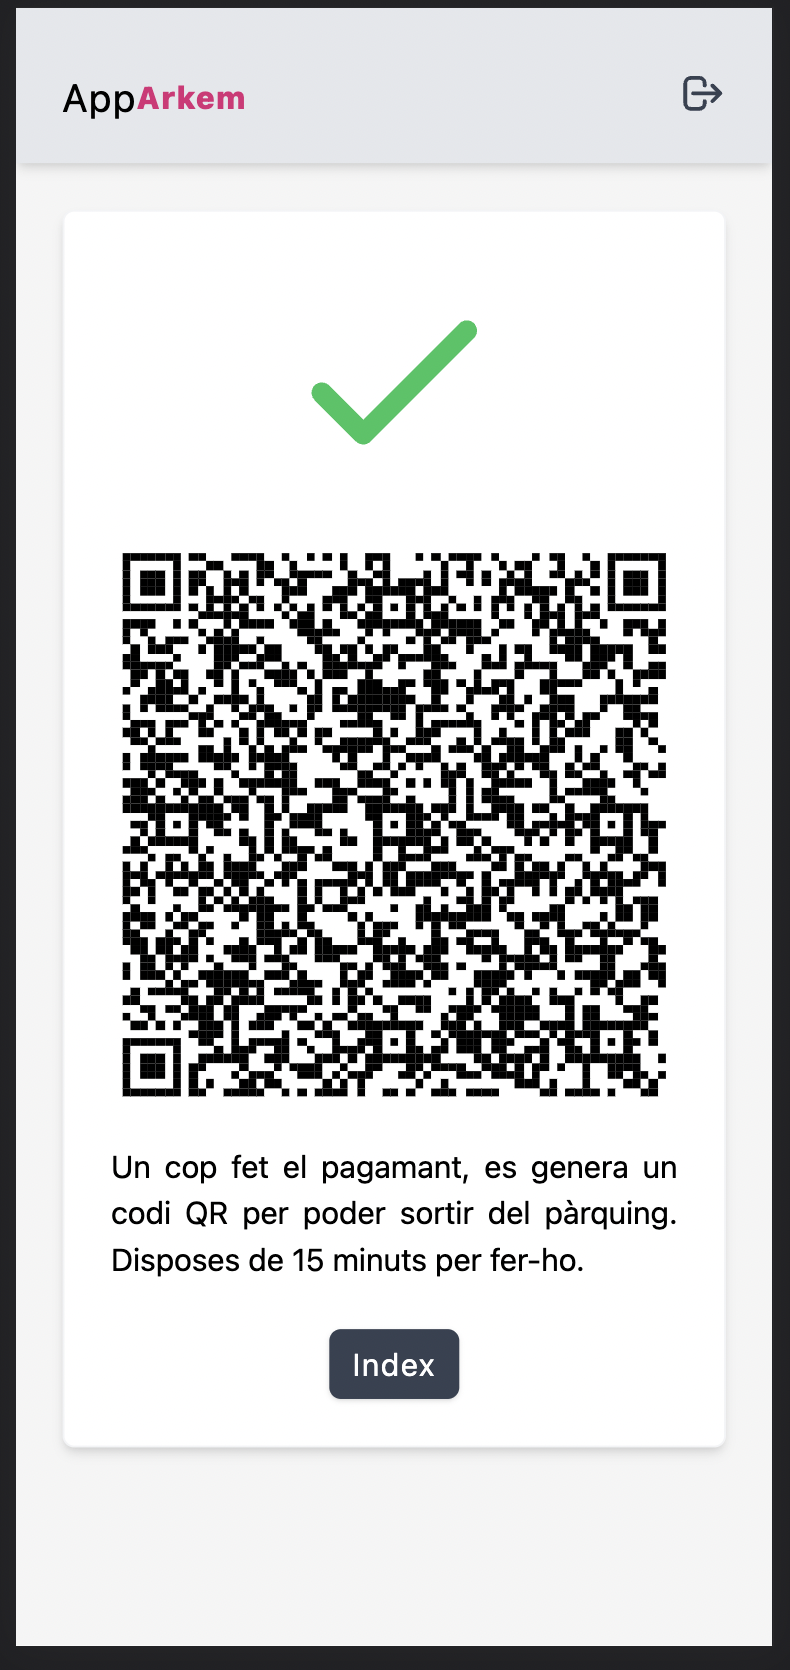
\includegraphics[scale=0.50]{Fotos/pantalla7_pagament_success.png}
    \end{center}
    \caption{Pantalla del pagament validat}
    \label{fig:payment_success_photo}
\end{figure}

\begin{figure}[H]
    \begin{center}
        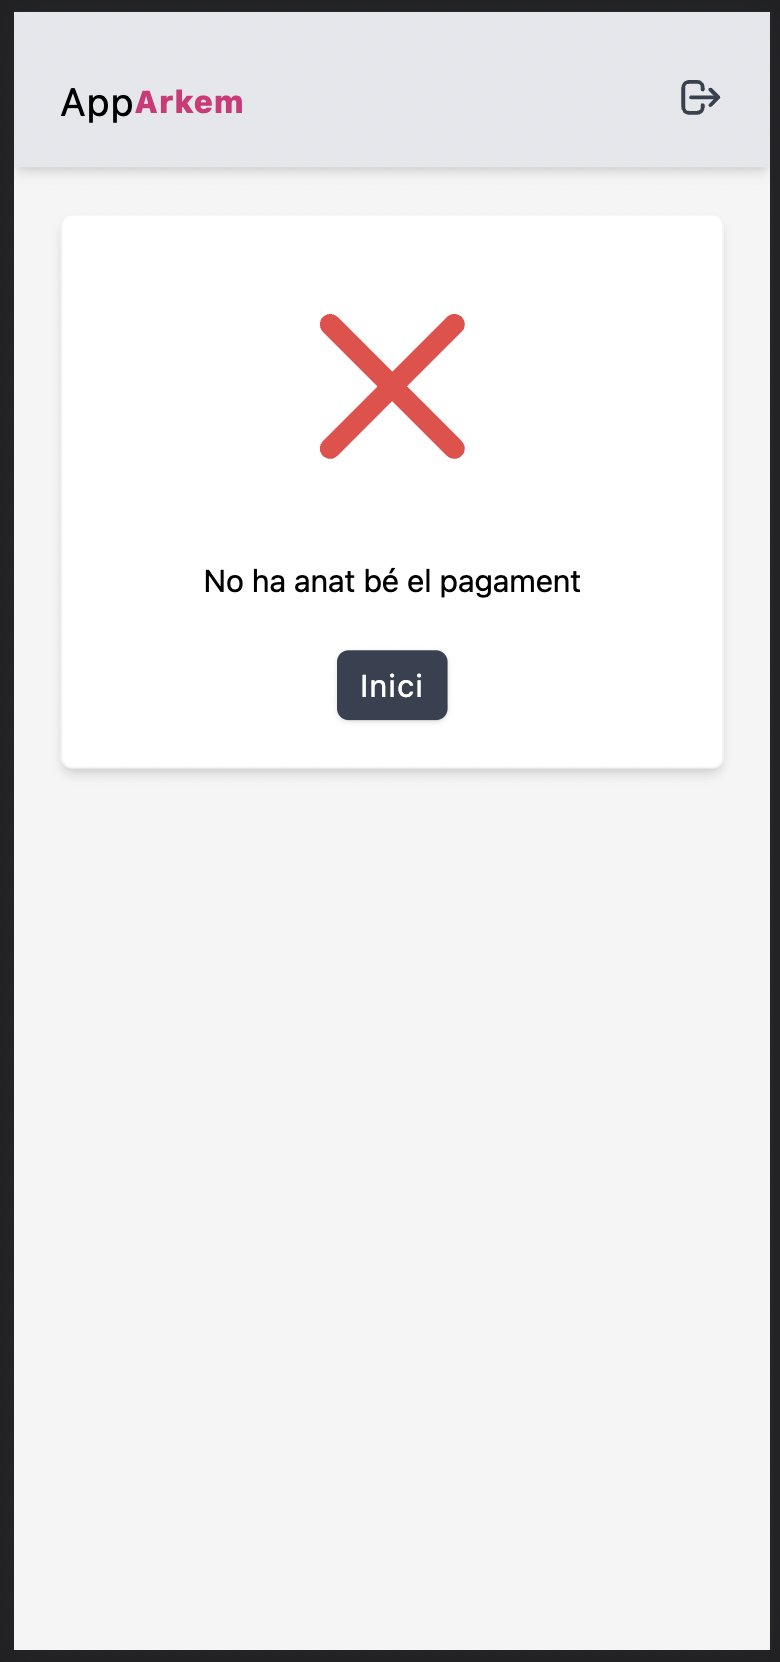
\includegraphics[scale=0.50]{Fotos/pantalla6_pagamanet_cancel.png}
    \end{center}
    \caption{Pantalla del pagament cance\l.lat}
    \label{fig:payment_cancel_photo}
\end{figure}

\begin{figure}[H]
    \begin{center}
        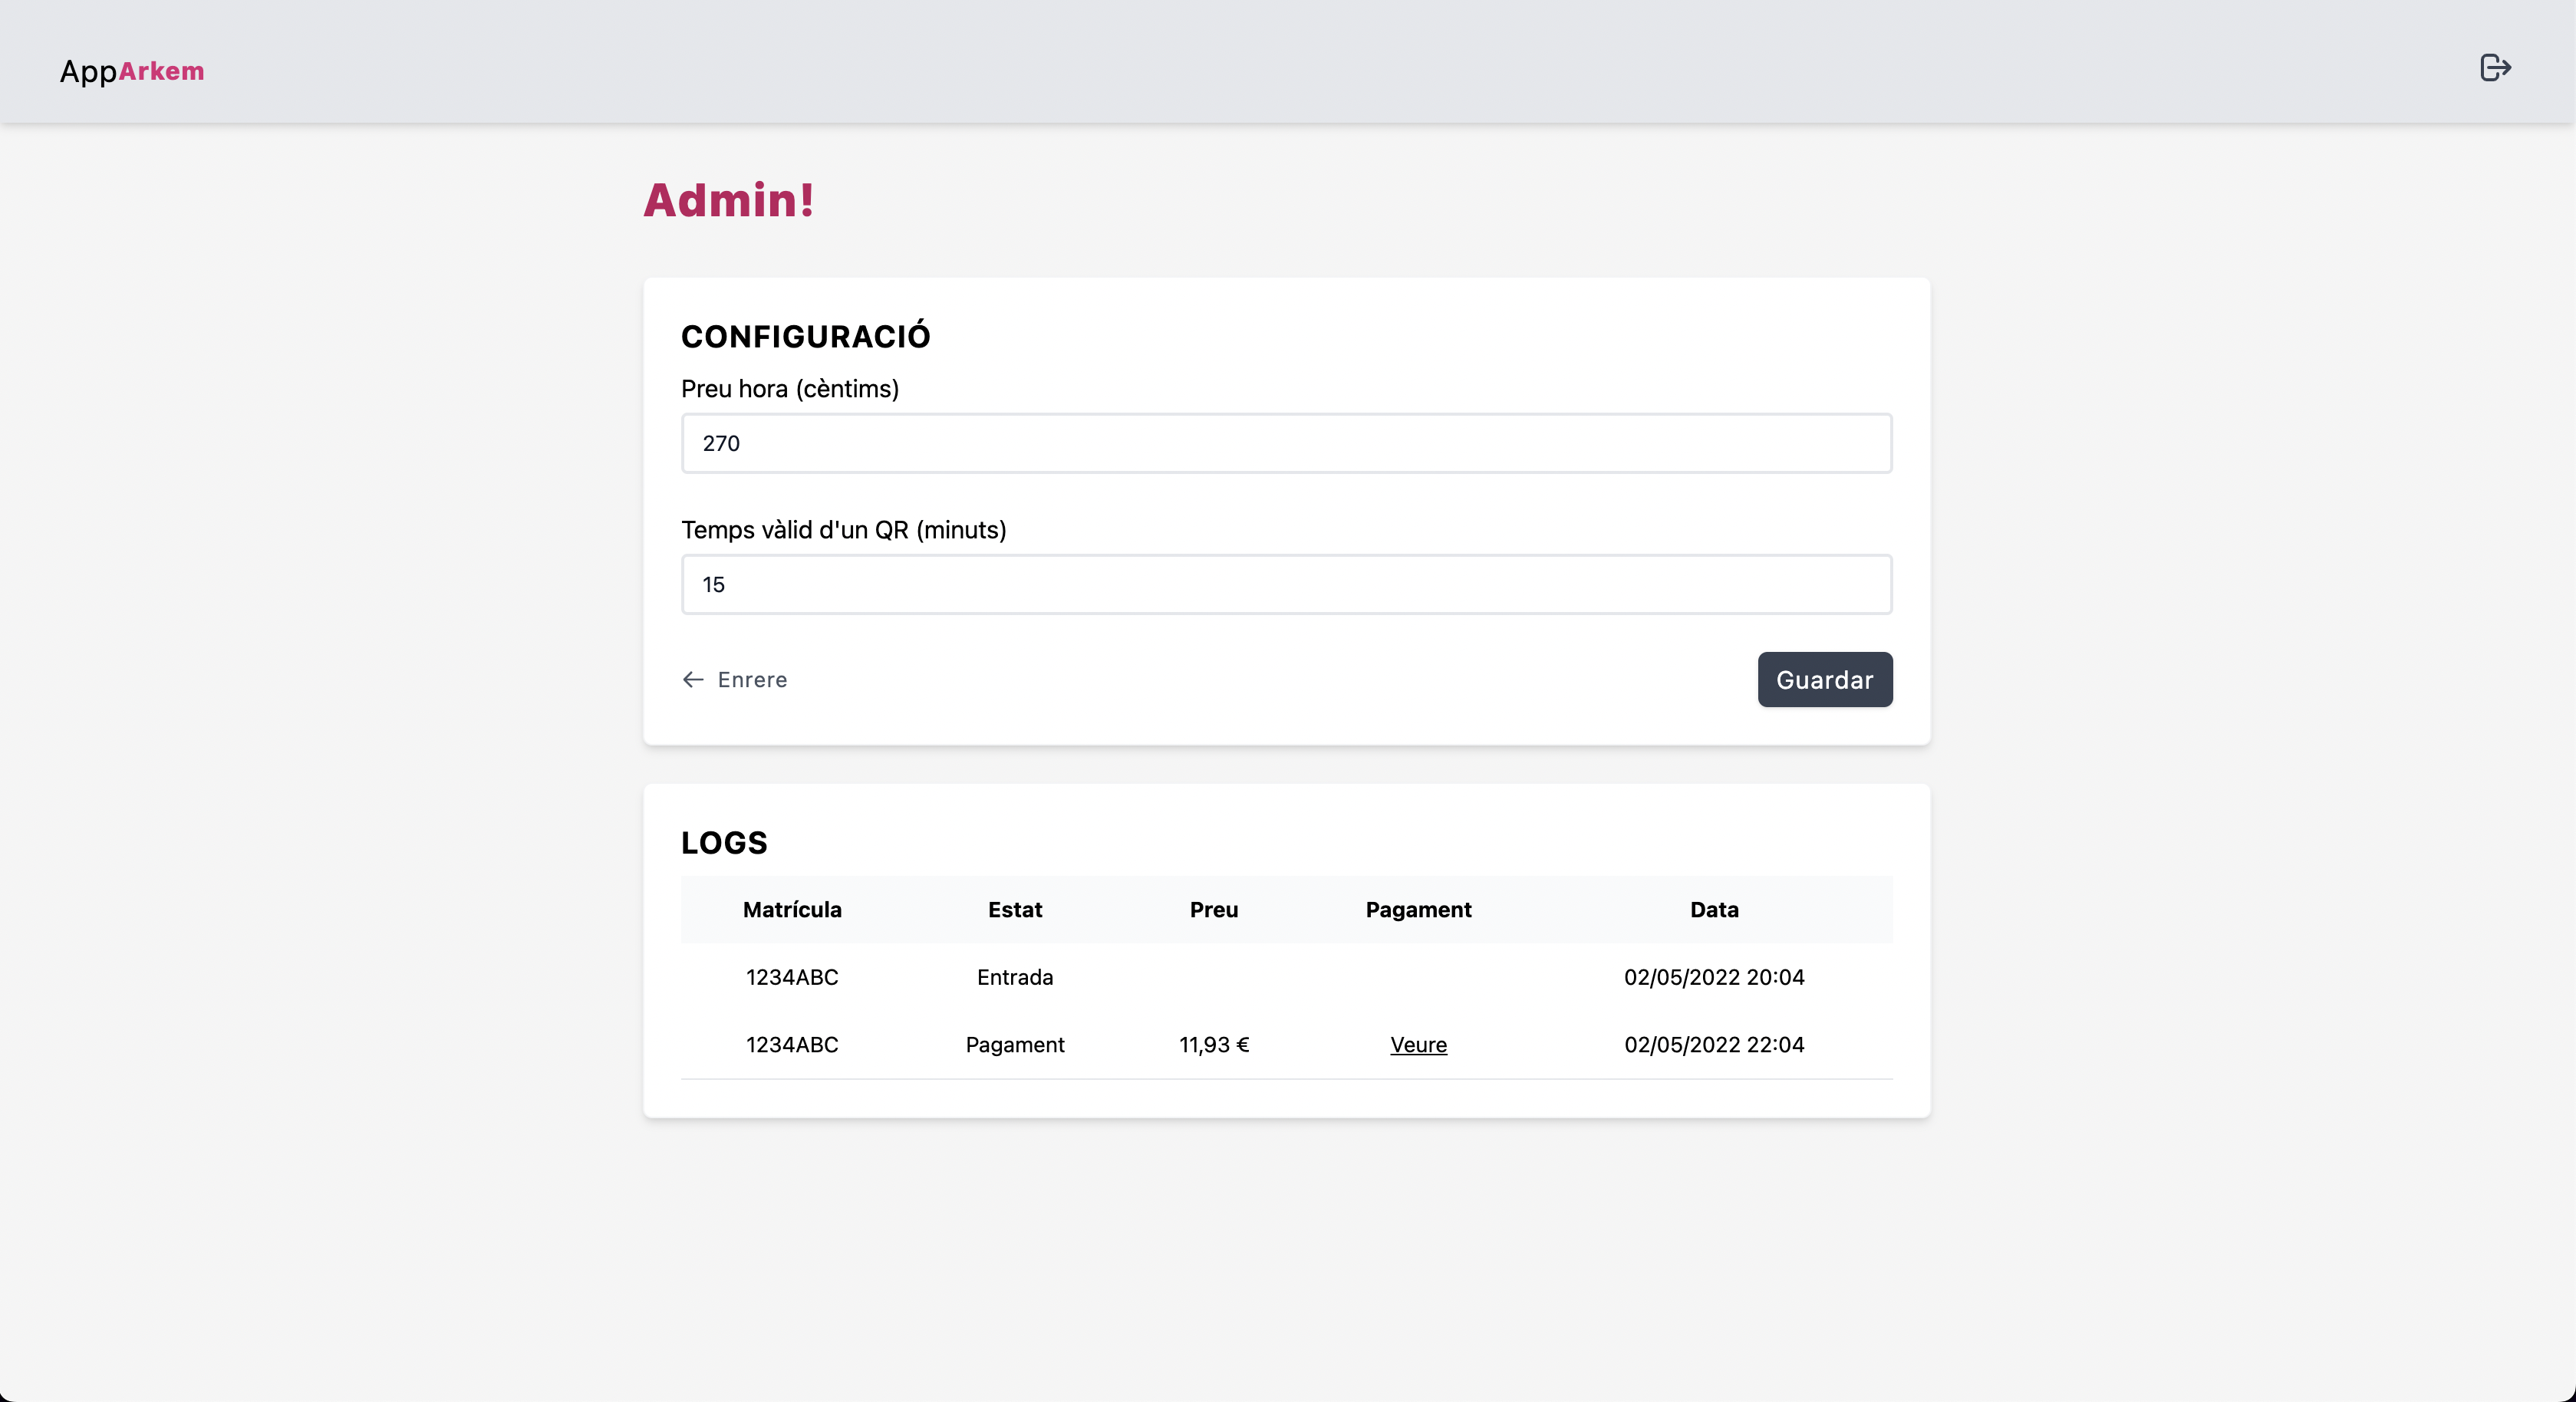
\includegraphics[scale=0.25]{Fotos/pantalla12_admin.png}
    \end{center}
    \caption{Pantalla panell d'administració}
    \label{fig:admin_photo}
\end{figure}

\begin{figure}[H]
    \begin{center}
        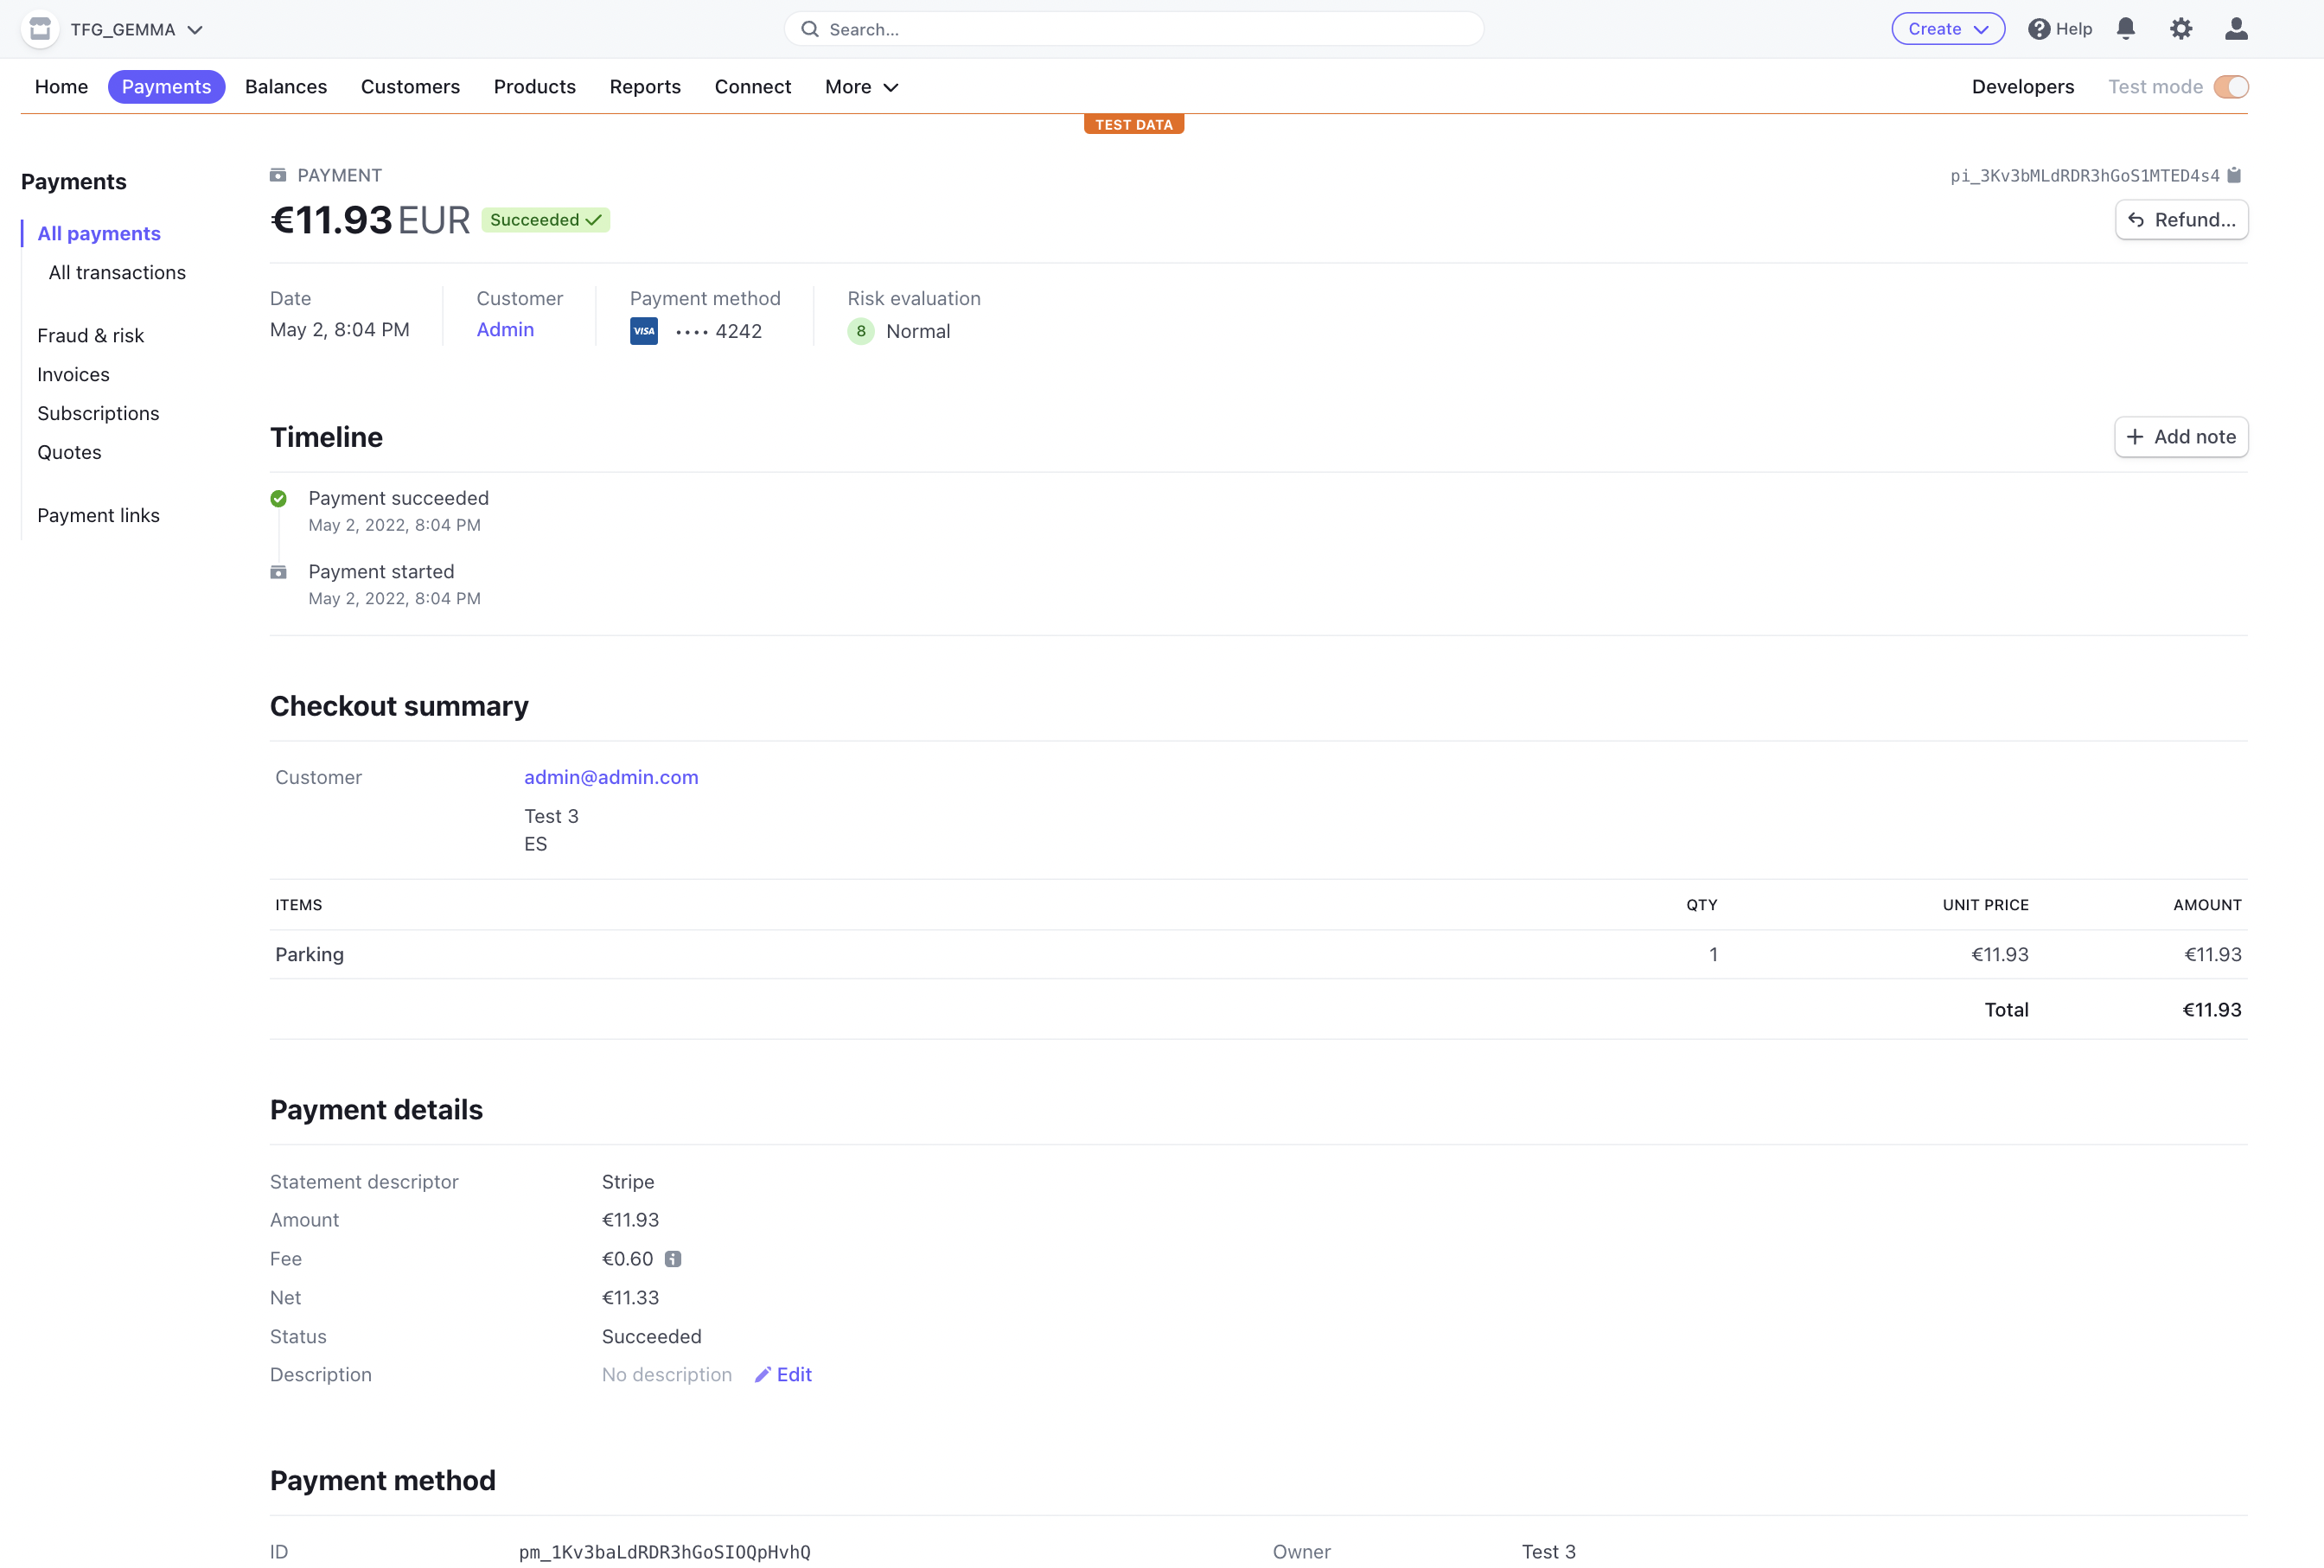
\includegraphics[scale=0.25]{Fotos/pantalla13_stripe.png}
    \end{center}
    \caption{Pantalla panell d'informació de pagament a \emph{Stripe}}
    \label{fig:stripe_info_photo}
\end{figure}

\newpage
\section{Alertes}

Per fer aquests \emph{PopUps}, l'aplicació ha fet servir la llibreria \texttt{SweetAlert2} \autocite{sweetalert2}

\begin{figure}[H]
    \begin{center}
        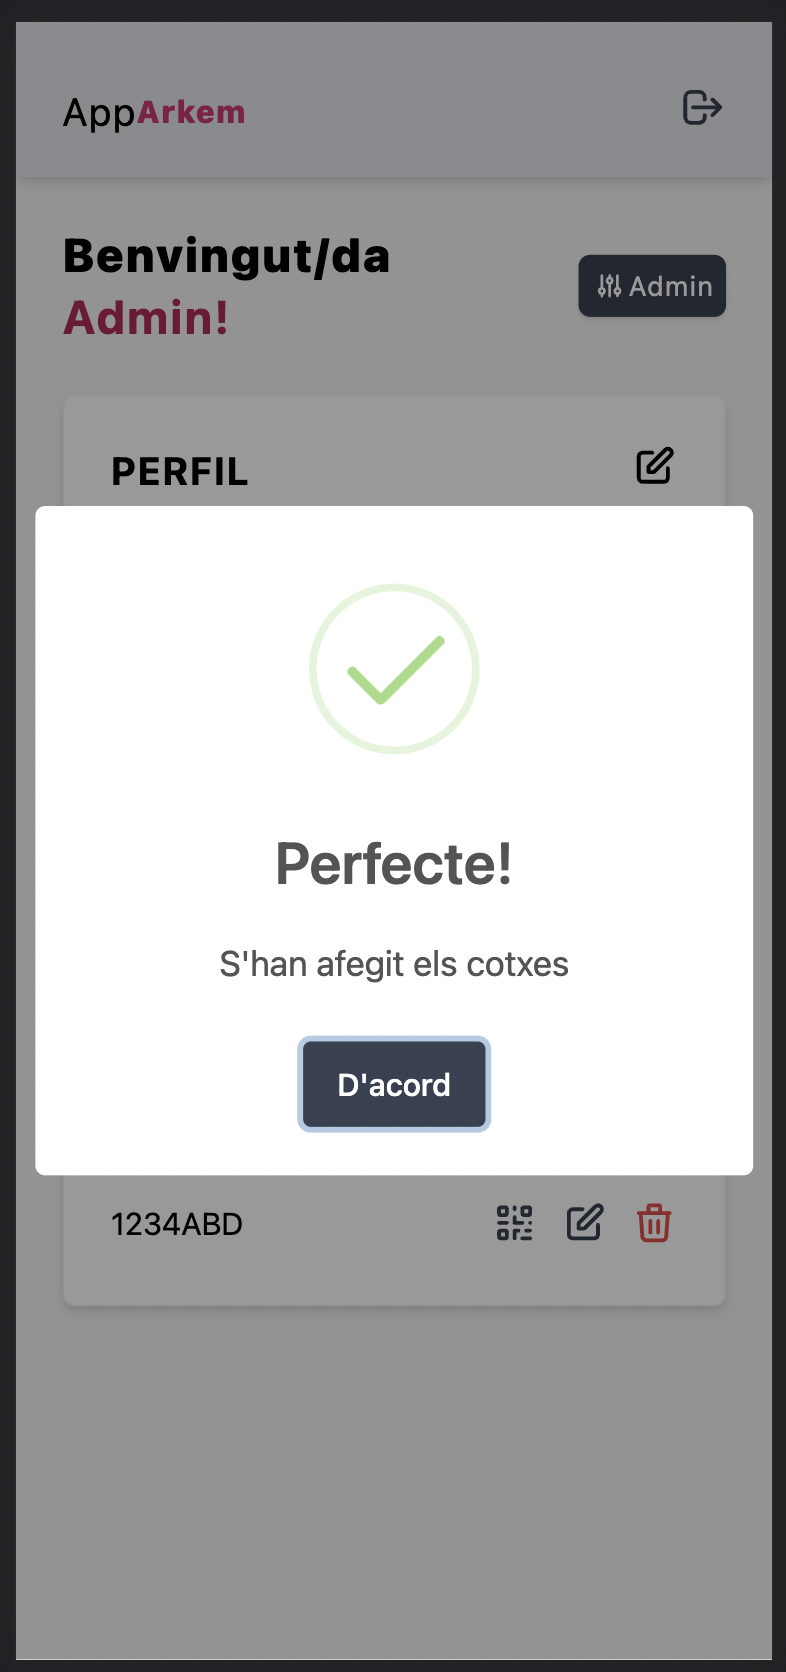
\includegraphics[scale=0.50]{Fotos/pantalla14_bannerCorrecte.png}
    \end{center}
    \caption{Alerta d'èxit}
    \label{fig:exit_alert}
\end{figure}

\begin{figure}[H]
    \begin{center}
        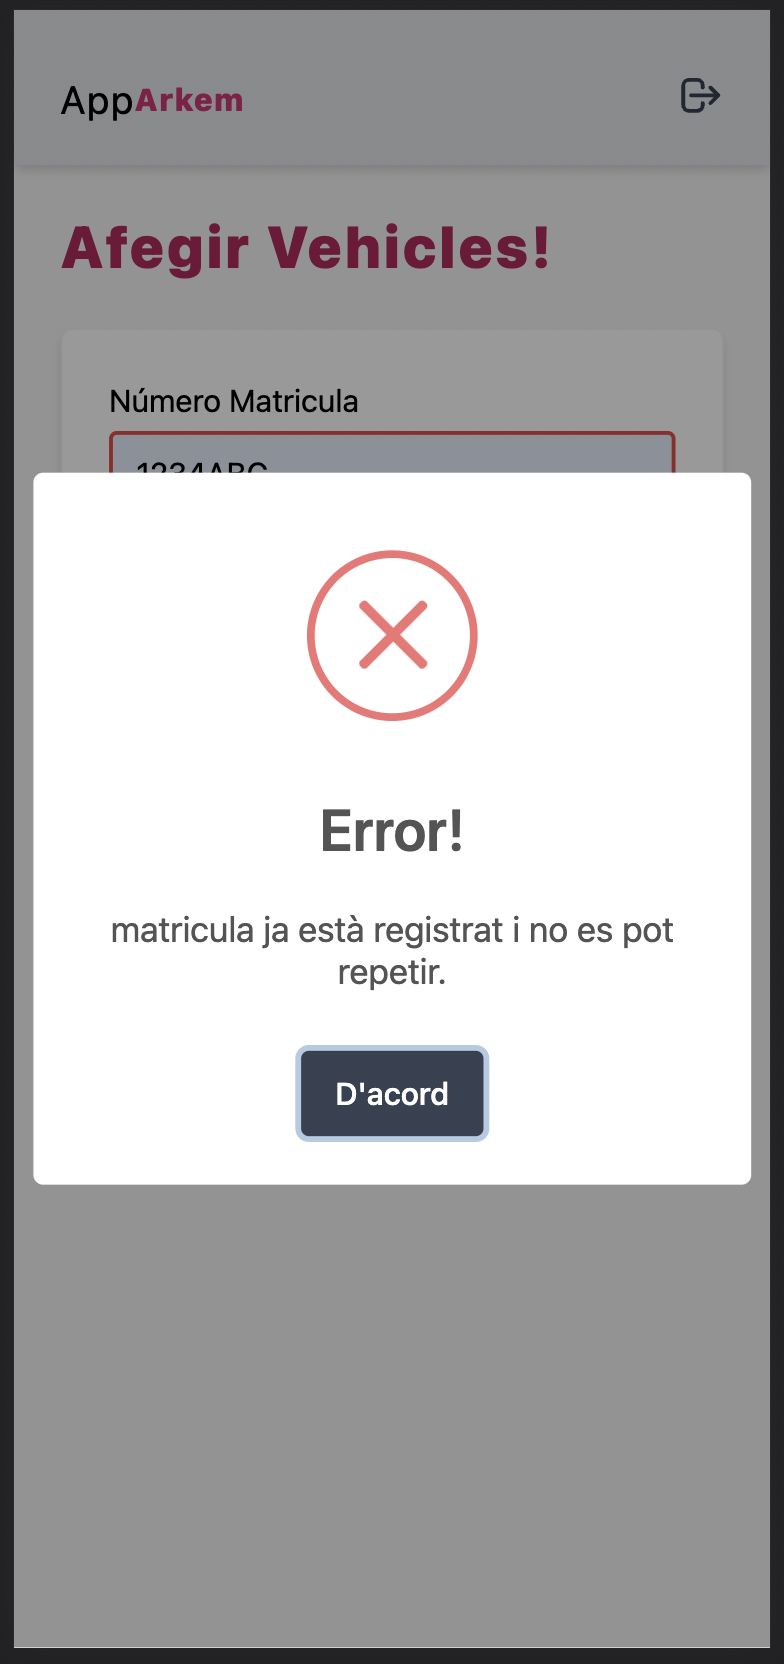
\includegraphics[scale=0.50]{Fotos/pantalla15_bannerError.png}
    \end{center}
    \caption{Alerta d'error}
    \label{fig:error_alert}
\end{figure}

\chapter{Enllaços a vídeos de l'aplicació}
Per veure el funcionament real del projecte es poden veure els següents vídeos:
\begin{itemize}
    \item Gravació del funcionament de l'aplicació. Compte d'administració inicia sessió,
    mostra com s'afegeixen cotxes de l'usuari \emph{Admin}. Finalment, clica el botó per entrar al
    pàrquing, on es genera un codi QR. Aquest codi QR és llegit per la barrera (Raspberry Pi).
    El servidor valida el codi QR, envia un esdeveniment (\emph{Web Sockets}) a l'aplicació on
    redirigeix a la pantalla d'informació.
    El vídeo és a \url{https://youtube.com/shorts/7SgkVWy9w_I?feature=share}
    \item Vídeo que mostra el funcionament de la barrera. On llegeix el codi QR generat per l'aplicació
    fa sonar el brunzidor. Fa la petició al servidor, es pot veure com el LED de color blau s'encén.
    La Raspberry Pi accedeix a apujar la barrera quan obté resposta del servidor. El LED verd fent pampallugues
    simbolitza que la barrera està pujant, un cop pujada el LED es queda encès un temps per poder entrar el
    vehicle dins del pàrquing. Finalment, la barrera baixa, també mostrant un LED blau fent pampallugues.
    Un cop ha baixat el LED es posa de color vermell.
    El vídeo és el següent \url{https://youtube.com/shorts/K7QQHMIinBw?feature=share}.
    \item L'usuari vol sortir del pàrquing, clica el botó de sortir i l'aplicació redirigeix l'usuari
    a la pantalla de pagaments. Inscriu una targeta de prova i quan el pagament és validat, l'aplicació el
    redirigeix a una pantalla on es genera el codi QR de sortida. La barrera el llegeix.
    \url{https://youtu.be/wfxZqMHwYiQ}
    \item La barrera llegeix el codi QR per sortir del pàrquing. La barrera quan llegeix el codi
    QR sona el brunzidor, i quan fa la petició HTTP ho mostra amb el LED blau. Quan ha rebut la resposta del servidor
    apuja la barrera perquè l'usuari pugui sortir del pàrquing i finalment baixa la barrera.
    \url{https://youtube.com/shorts/7WrHquP0_tA?feature=share}.
    \item L'usuari mostra a la barrera un codi QR que no és el bo. La barrera quan llegeix el codi
    QR sona un \emph{Bzz} el brunzidor, i quan fa la petició HTTP ho mostra amb el LED blau.
    La resposta del servidor no és satisfactòria, per tant, la barrera mostra amb un pampallugueig de color vermell que alguna
    cosa no ha funcionat correctament \url{https://youtube.com/shorts/xCrC1VhblQo?feature=share}.
    \item Gravació de la pantalla d'administració. Mostra dels \emph{Logs} i de la pàgina de pagament de\emph{Stripe}.
    \url{https://youtu.be/p9qcisBsLWI}
\end{itemize}

\chapter{Trobar AppArkem}

L'aplicació es pot trobar a \url{https://github.com/GemmaGuilella/TFG_GEMMA}.

Les carpetes s'organitzen per:
\begin{enumerate}
    \item \texttt{my-parking}: La carpeta on hi ha l'aplicació \emph{front-end}.
    \item \texttt{Parking}: Aquesta carpeta hi ha el servidor de \emph{Laravel}, és a dir la part de \emph{back-end}.
    \item \texttt{thesis-master}: Generador de la memòria del TFG.
    \item \texttt{Raspberry Pi}: on hi ha el codi client de la Raspberry Pi.
\end{enumerate}

\end{document}
